% DOCUMENT FORMAT ======================= -*- mode: LaTeX; coding: utf-8 -*- ===

\documentclass[diploma]{softlab-thesis}


% PACKAGE SETTINGS =============================================================

\usepackage{fontspec}
\usepackage{amsmath}
\usepackage{amsfonts}
\usepackage{multirow}
\usepackage{array}
\usepackage{mdwlist}
\usepackage{subfig}
\usepackage{floatrow}
\usepackage{float}
\usepackage{verbatim}
\usepackage{color}
\usepackage{graphicx}
\usepackage{xunicode}
\usepackage{xltxtra}
\usepackage{url}
%\usepackage{dsfont}
%\usepackage{microtype}
\usepackage{hyphenat}
\usepackage{multicol}
\usepackage{wrapfig}
\usepackage{lipsum}
\usepackage{listings}
\usepackage{paralist}
\usepackage{ulem}
\usepackage{tocvsec2}
\usepackage{url}
\usepackage[toc,page]{appendix}
% FONT SETTINGS ===============================================================

%\setromanfont[Mapping=tex-text]{CMU Serif}
%%\setromanfont[Mapping=tex-text]{CMU Sans Serif} % temporary change until printing
%%\setsansfont[Mapping=tex-text]{CMU Sans Serif}
%%\setmonofont[Mapping=tex-text]{CMU Typewriter Text}
%\setmainfont[Mapping=tex-text]{CMU Serif}
%%\setmainfont[Mapping=tex-text]{CMU Sans Serif}  % temporary change until printing

%\setromanfont[Mapping=tex-text,ExternalLocation=fonts/]{cmunrm.otf}
%\setsansfont[Mapping=tex-text,ExternalLocation=fonts/]{cmunss.otf}
%\setmonofont[Mapping=tex-text,ExternalLocation=fonts/]{cmuntt.otf}
%\setmainfont[Mapping=tex-text, ExternalLocation=fonts/]{cmunss.otf}

\defaultfontfeatures{Mapping=tex-text}
%\setromanfont{Linux Libertine O}
\setromanfont{DroidSerif}

% CUSTOM COLORS ===============================================================

\definecolor{gray}{rgb}{0.5,0.5,0.5}
\definecolor{darkgreen}{rgb}{0.0,0.5,0.0}
\definecolor{mygreen}{rgb}{0,0.6,0}
\definecolor{mygray}{rgb}{0.5,0.5,0.5}
\definecolor{mymauve}{rgb}{0.58,0,0.82}
\definecolor{myorange}{RGB}{246,177,50}

% CUSTOM COMMANDS =============================================================

\newcommand\fixme{\textrm{\textbf{\textcolor{red}{FIXME: }}}}
\newcommand\todo{\textrm{\textbf{\textcolor{myorange}{TODO: }}}}
\newcommand\mytilde{\raise.17ex\hbox{$\scriptstyle\sim$}}
\newcommand\okeanos{\textbf{\raise.17ex\hbox{$\scriptstyle\sim$}okeanos }}


% Layout macros
\newcommand\spa[1]{\; #1 \;}

% Font macros
\newcommand\resfont[1]{\ensuremath{\mathtt{#1}}}

% Mathematical macros
\newcommand\setmap[3]{#1\{#2 \mapsto #3\}}
\newcommand\getmap[3]{(#2 \mapsto #3) \in #1}
\newcommand\tuple[2]{\ensuremath{\langle#1, #2\rangle}}
\newcommand\mfrac[2]{\ensuremath{\dfrac{#1}{#2}}}
\newcommand\nequiv[2]{\ensuremath{#1 \not\equiv #2}}

% Core Ruby Operational Semantics letter bindings
\newcommand\mem{\mu}

% Core Ruby Operational Semantics low level macros
\newcommand\state[2]{(#1, #2)}
\newcommand\transition[1]{\ensuremath{\overset{#1, c*}{\rightarrow}}}
\newcommand\range[2]{#1, ..., #2}
\newcommand\midrange[5]{\range{#1}{#2}, #3, \range{#4}{#5}}

% Core Ruby Operational Semantics high level macros
\newcommand\operation[5]{\ensuremath{\state{#1}{#2} \transition{#3} \state{#4}{#5}}}
\newcommand\propagation[2]{\operation{#1}{\mem}{#2}{#1'}{\mem'}}

% Core Ruby specific Operational Semantics macros
\newcommand\semicolon[2]{#1; \; #2}
\newcommand\assign[2]{#1 = #2}
\newcommand\mcall[3]{#1.\texttt{#2}(#3)}
\newcommand\ifte[3]{\resfont{if} \; #1 \; \resfont{then} \; #2 \; \resfont{else} \; #3}
\newcommand\newclass[2]{#1.\resfont{new}(#2)}
\newcommand\methoddef[3]{\resfont{def} \; #1(#2) = #3}
\newcommand\classdef[2]{\resfont{class} \; #1 = #2}
\newcommand\with[3]{with \; \tuple{#1}{#2} \; do \; #3}

% Success Typing macros
\newcommand\ssub{\sqsubseteq\_S}

% Core Ruby Success Typing letter bindings
\newcommand\classlist{\Delta}
\newcommand\envir{\Gamma}
\newcommand\fields{\Phi}
\newcommand\currclass{l}

% Core Ruby Success Typing inferencing macros
\newcommand\stinfer[5]{\classlist; \; #1; \; \fields \; \underset{\currclass}{\vdash} \; #2: #3 \; \& \; #4; \; #5}


%%%%%%%%%%%%%%%%%%%%%%%%%%% CACHED STUFF %%%%%%%%%%%%%%%%%%%%%%%%%%%

\newcommand\xcache{\texttt{xcache} }

%%%%%%%%%%%%%%%%%%%%%%%%%%% HASKELL STUFF %%%%%%%%%%%%%%%%%%%%%%%%%%%

%\newcommand\typerep[1]{\ensuremath{#1}}
\newcommand\typerep[1]{\lstinline[basicstyle=\normalsize\ttfamily,keywords={}]|#1|}
\newcommand\typefootrep[1]{\textbf{\lstinline[basicstyle=\footnotesize\ttfamily,keywords={}]|#1|}}
% \newcommand\ttyperep[1]{\typerep{#1}}
% \newcommand\mtyperep[1]{\mbox{\typerep{#1}}}

% Arrow types
\newcommand\typeto[2]{\typerep{#1} \typerep{->} \typerep{#2}}
\newcommand\typetotwo[3]{\ensuremath{\typerep{#1} \typerep{->}
                                     \typerep{#2} \typerep{->}
                                     \typerep{#3}}}

\newcommand\tyconapone[2]{\ensuremath{\mbox{\typerep{#1}} \:\: \mbox{#2}}}
\newcommand\tyconaponeC[2]{\ensuremath{\mbox{\typerep{#1}} \:\: \mbox{\typerep{#2}}}}
% \newcommand\tyconapone[2]{\typerep{#1} $\:$ \typerep{#2}}

\newcommand\tyconaptwo[3]{\ensuremath{\mbox{\typerep{#1}} \:\: \mbox{#2} \:\: \mbox{#3}}}


% FIGURE SETUP ===============================================================

\newcommand\diagram[2]{
	\begin{figure}[h!]
		\centering
		\includegraphics[width=\textwidth,height=\textheight,keepaspectratio]
		{diagrams/#2}
		\caption{#1}
		\label{fig:#2}
	\end{figure}
}

\newcommand\diagramscale[3]{
	\begin{figure}[h!]
		\centering
		\includegraphics[scale={#3}]
		{diagrams/#2}
		\caption{#1}
		\label{fig:#2}
	\end{figure}
}
\newcommand\diagramstrict[2]{
	\begin{figure}[H]
		\centering
		\includegraphics[keepaspectratio]
		{diagrams/#2}
		\caption{#1}
		\label{fig:#2}
	\end{figure}
}


% SPELLING =====================================================================

% CODE HIGHLIGHTING ============================================================

% Define common settings for code listings

\lstset{
	backgroundcolor=\color{white},
	basicstyle=\small\ttfamily,		% style for code
	breakatwhitespace=false,        % sets if automatic breaks should only
					% happen at whitespace
	breaklines=true,                % sets automatic line breaking
	captionpos=b,                   % sets the caption-position to bottom
	commentstyle=\color{mygreen},   % style for comments
	escapeinside={\%*}{*)},         % if you want to add LaTeX within your code
	frame=single,                   % adds a frame around the code
	keepspaces=true,                % keeps spaces in text, useful for
	%keywordstyle=\color{blue}\bfseries,
					% keyword style
	numbers=left,
	numbersep=5pt,                  % how far the line-numbers are from the
					% code
	numberstyle=\tiny\color{mygray},% style for line-numbers
	rulecolor=\color{black},
	stepnumber=1,                   % the step between two line-numbers. If
					% it's 1, each line will be numbered
	stringstyle=\color{mymauve},    % style for strings
	tabsize=2,                      % sets default tabsize to 2 spaces
}

\lstdefinestyle{plain}
{
	stepnumber=0
}

% Create new commands for simpler usage

\newcommand\plaintext[2]{
	\lstinputlisting[style=plain, caption={#1},
	label=lst:#2]{src/#2}
}

% CHANGE MATH FONT ============================================================

% HYPERREF MUST BE LAST =======================================================

\usepackage[xetex,colorlinks=true,linkcolor=blue,citecolor=darkgreen]{hyperref}

% DOCUMENT INFORMATION =========================================================

\title{Πιθανοτικές επιθέσεις σε συμπιεσμένα, κρυπτογραφημένα πρωτόκολλα}

% ===============> FIXME
\author{Δημήτριος Καρακώστας}
\authoren{Dimitrios Karakostas}
\datedefense{11}{1}{2016}
\supervisor{Αριστείδης Παγουρτζής}
\supervisorpos{Αναπληρωτής Καθηγητής ΕΜΠ}
\committeeone{Αριστείδης Παγουρτζής}
\committeeonepos{Αναπληρωτής Καθηγητής ΕΜΠ}
\committeetwo{Δημήτριος Φωτάκης}
\committeetwopos{Επίκουρος Καθηγητής ΕΜΠ}
\committeethree{Άγγελος Κιαγιάς}
\committeethreepos{Επίκουρος Καθηγητής ΕΚΠΑ}
\hypersetup{
	pdftitle={},
	pdfauthor={test},
	pdfsubject={},
	pdfkeywords={}
}


% MAIN DOCUMENT ================================================================

\begin{document}

\frontmatter
\maketitle

\def\templen{\parindent}
\setlength{\parindent}{0pt}
\setlength{\parskip}{1.5ex plus 0.5ex minus 0.2ex}
\begin{abstractgr}

Η ασφάλεια είναι ένα από τα βασικά χαρακτηριστικά κάθε σύγχρονου υπολογιστικού
συστήματος. Η παρούσα εργασία ερευνά επιθέσεις πάνω σε συμπιεσμένα
κρυπτογραφημένα πρωτόκολλα.

Συγκεκριμένα, προτείνεται μια νέα ιδιότητα που χαρακτηρίζει κρυπτοσυστήματα, η
μη-διακρισιμότητα ενάντια σε επιθέσεις μερικώς επιλεγμένου κειμένου (IND-PCPA),
καθώς και ένα μοντέλο επίθεσης που χρησιμοποιεί αυτή την ιδιότητα. Προκειμένου
να ξεπεραστούν εμπόδια που παρουσιάζονται σε συστήματα του πραγματικού κόσμου,
προτείνονται στατιστικές μέθοδοι, οι οποίες βελτιώνουν την επίδοση και
εγκυρότητα της επίθεσης.

Τα πειράματα που διεξήχθησαν κατά τη διάρκεια της εργασίας αφορούσαν σε δύο
ευρέως χρησιμοποιούμενα συστήματα, το Facebook Chat και το Gmail, για την
επίτευξη των οποίων χρησιμοποιήθηκε λογισμικό, το οποίο αναπτύχθηκε σε Python
για τους σκοπούς αυτής της εργασίας. Τα πειράματα έγιναν σε συνθήκες εργαστηρίου
και απέδειξαν ότι τα δύο αυτά συστήματα δεν είναι IND-PCPA, όσον αφορά
συγκεκριμένους τύπους μυστικών.

Τέλος, προτείνονται καινοτόμες τεχνικές, οι οποίες θα οδηγήσουν σε πλήρη
αντιμετώπιση επιθέσεων που ακολουθούν το μοντέλο που προτείνεται, όπως η
επίθεση που παρουσιάστηκε στην παρούσα εργασία.

\end{abstractgr}

\begin{abstracten}

Security is a fundamental aspect of every modern system. This work investigates
attacks on compressed encrypted protocols.

A new property of cryptosystems is proposed, cited Indistinguishability under
Partially Chosen Plaintext Attack (IND-PCPA), along with an attack model that
works under such a mechanism. In order to bypass obstacles of real-world
systems, statistical methods were proposed, to improve the performance and
validity of the attack.

Experiments were conducted on two widely used systems, Facebook Chat and Gmail, using
a Python framework, that was implemented for the purpose of this paper. Results
in lab environment revealed that those two systems are not IND-PCPA, regarding
certain specified types of secrets.

Finally, novel techniques were proposed, that could lead to complete mitigation
of attacks that follow the proposed model.

\end{abstracten}


\setlength{\parindent}{\templen}
\setlength{\parskip}{0pt}
\tableofcontents
\listoffigures
%\listoftables
\renewcommand{\lstlistlistingname}{List of Listings}
\lstlistoflistings % changed the title above

\mainmatter
% moved these two commands here so that they don't influence the toc
\setlength{\parindent}{0pt}
\setlength{\parskip}{1.5ex plus 0.5ex minus 0.2ex}

\renewcommand\floatpagefraction{.7}

\chapter{Εισαγωγή}\label{ch:intro}
\epigraph{\itshape Even if you're not doing anything wrong, you are being watched and
recorded.}{---Edward Snowden}

\section{Εισαγωγή}\label{sec:intro}

Το καλοκαίρι του 2013 επιβεβαιώθηκε αυτό που υπήρχε ως υποψία όλα τα προηγούμενα
χρόνια: οι συνομιλίες παρακολουθούνται και τα δεδομένα που ανταλλάσσονται μέσω
Διαδικτύου δεν είναι ασφαλή. Οι αποκαλύψεις Snowden άλλαξαν τον τρόπο με τον
οποίο αντιλαμβανόμαστε τη χρήση online υπηρεσιών και έστρεψαν πολλούς ερευνητές
και χρήστες στην αναζήτηση λύσεων ώστε οι επικοινωνίες να γίνουν πιο ασφαλείς
απέναντι σε κάθε είδους αντιπάλους.

Η παρούσα εργασία στοχεύει να αναδείξει αδυναμίες στα πρωτόκολλα που επιτρέπουν
την επικοινωνία μέσω Διαδικτύου και μέσω της δημοσίευσής της να κινητοποιήσει
την κοινότητα ώστε να αντιμετωπιστούν αυτά τα προβλήματα.

Η έρευνά μας επικεντρώνεται σε επιθέσεις που εκμεταλλεύονται τους αλγόριθμους
συμπίεσης που χρησιμοποιούνται πάνω στα δεδομένα που ανταλλάσσονται, προτού αυτά
κρυπτογραφηθούν και αποσταλούν. Συγκεκριμένα, επεκτείνουμε υπάρχοντα μο-ντέλα,
όπως το BREACH, ώστε να καταδείξουμε πως πρωτόκολλα τα οποία θεωρούνται σήμερα
απολύτως ασφαλή είναι πρακτικά τρωτά σε παρόμοιες επιθέσεις.

Κατά τη διάρκεια της έρευνάς μας επικεντρωθήκαμε στο λογισμικό συμπίεσης gzip,
το οποίο εφαρμόζει τον αλγόριθμο DEFLATE, ο οποίος με τη σειρά του αποτελεί
συνδυασμό των αλγορίθμων συμπίεσης Huffman και LZ77. Συγκεκριμένα, η επίθεση
εκμεταλλεύε-ται την ανάλυση που κάνει ο LZ77 πάνω στο καθαρό κείμενο, ενώ
αντίθετα η ύπαρξη συμπίεσης Huffman εμποδίζει την εκτέλεση. Παρότι δεν ελέγξαμε
άλλους αλγόριθμους ή εμπορικές εφαρμογές συμπίεσης, είναι αρκετά ασφαλές να
υποθέσουμε πως αλγόριθ-μοι που ακολουθούν όμοιες τεχνικές είναι δυνητικά στόχοι
για παρόμοιες επιθέσεις.

Το πιο διαδεδομένο πρωτόκολλο ανταλλαγής δεδομένων στο Διαδίκτυο είναι το HTTP
(Hyper-Text Transfer Protocol). Είναι ευρέως αποδεκτό πως δεδομένα που
στέλνονται μέσω απλού HTTP και δεν είναι κρυπτογραφημένα θα πρέπει να
θεωρούνται ανασφαλή ως προς την ακεραιότητα και την αυθεντικότητά τους. Το κενό
στην ασφάλεια που αφήνει το απλό HTTP ήρθε να συμπληρώσει αρχικά το SSL (Secure
Socket Layer) και στη συνέχεια το TLS (Transport Layer Security). Το TLS
εισάγεται ως ένα επίπεδο δικτύου πριν το επίπεδο εφαρμογής και επιβάλλει την
κρυπτογράφηση των δεδομένων πριν αυτά σταλούν στο Διαδίκτυο.

Οι αλγόριθμοι κρυπτογράφησης που χρησιμοποιούνται εν γένει μπορούν να χωριστούν
σε δύο κύριες κατηγορίες: ροής και δέσμης. Στην πρώτη περίπτωση, τα δεδομένα
κρυ-πτογραφούνται ως μια συνεχής ροή, ενώ στη δεύτερη περίπτωση χωρίζονται σε
δέσμες ίσου μεγέθους και κρυπτογραφείται κάθε δέσμη χωριστά. Σε περίπτωση που τα
δεδομέ-να δεν κατανέμονται με ακρίβεια σε δέσμες, εισάγεται τεχνητός θόρυβος
ώστε να επιτευχθεί το επιθυμητό μέγεθος.

Ο κυριότερος αλγόριθμος ροής είναι ο RC4, ο οποίος πλέον θεωρείται ανασφαλής και
αποφεύγεται η χρήση του. Από την άλλη πλευρά, ο πιο διαδεδομένος αλγόριθμος
δέσμης είναι ο AES, ο οποίος χρησιμοποιείται σε διάφορες παραλλαγές από την
πλειοψηφία των συστημάτων. Η χρήση αλγορίθμων ροής καθιστά την επίθεση που
περιγράφουμε πολύ ευκολότερη, καθώς μειώνεται η ύπαρξη θορύβου που μπορεί να
επηρεάσει τα αποτελέσματα. Ωστόσο, κατά τη διάρκεια της έρευνάς μας, διαπιστώσαμε πως η
χρήση του AES δεν εξασφαλίζει απόλυτη ασφάλεια και υπό προϋποθέσεις είναι δυνατό
δεδομέ-να που ανταλλάσσονται με αυτές τις μεθόδους να υποκλαπούν.

Για να το επιτύχουμε αυτό έπρεπε αρχικά να μοντελοποιήσουμε την επίθεσή μας. Για
το σκοπό αυτό ορίσαμε μια νέα κρυπτογραφική ιδιότητα, την οποία ονομάζουμε
μη-διακρισιμότητα ενάντια σε επιθέσεις μερικώς επιλεγμένου κειμένου (IND-PCPA). Όμοιες
ιδιότητες, όπως IND-CPA, IND-CCA κ.ά, είναι ορισμένες στη βιβλιογραφία και
χρησιμοποιούνται ευρέως στην ανάλυση κρυπτοσυστημάτων. Η εισαγωγή της IND-PCPA
στοχεύει στην επέκταση των αναλύσεων ώστε να καλύπτουν επιθέσεις όπως αυτή που
αναπτύσσεται στην παρούσα εργασία.

Η επιτυχία της επίθεσης προϋποθέτει το σύστημα το οποίο αναλύεται να παρουσιάζει
συγκεκριμένα χαρακτηριστικά-παθογένειες. Η επίλυση των παθογενειών είναι
δεδομέ-νο πως βοηθάει σε σημαντικό βαθμό στην αντιμετώπιση της επίθεσης. Συνεπώς,
είναι σημαντικό να μοντελοποιήσουμε την επίθεση και να ορίσουμε τα
χαρακτηριστικά της, προτού επιχειρήσουμε να βρούμε τρόπους αντιμετώπισής της.

Η επίθεση που ερευνάται είναι επέκταση γνωστών μοντέλων, όπως αναφέρθηκε. Ωστό-σο
η ανάλυσή μας οδηγεί σε χαλάρωση των απαιτήσεων που θεωρούνταν δεδομένες και,
κατά συνέπεια, στοχεύει σε μεγαλύτερο εύρος συστημάτων. Είναι εμφανές πως
σε οποιοδήποτε σύστημα ικανοποιούνται οι απαιτήσεις που ορίζουμε η επίθεση είναι
δυνητικά εφικτή, συνεπώς το σύστημα θα πρέπει να θεωρείται ανασφαλές.

Στην παρούσα εργασία περιγράφονται αδυναμίες σε δύο εφαρμογές που
χρησιμοποιού-νται από μεγάλο ποσοστό χρηστών του Διαδικτύου. Η πρώτη είναι η
υπηρεσία chat του Facebook, όπου αναλύουμε τον τρόπο με τον οποίο προσωπικά
μηνύματα κάποιου χρήστη μπορούν να υποκλαπούν. Η δεύτερη είναι η υπηρεσία email
της Google, το Gmail. Σε αυτή την περίπτωση, παρουσιάζουμε πώς μπορεί κάποιος
επιτιθέμενος να αποκτήσει τον έλεγχο του λογαριασμού ενός χρήστη ώστε να είναι
σε θέση να υποδυθεί τον χρήστη, καθώς και να υποκλέψει δεδομένα που
ανταλλάχθησαν μέσω mail.

Για την εκτέλεση των πειραμάτων αναπτύξαμε λογισμικό σε επίπεδο
proof-of-concept, το οποίο μπορεί να χρησιμοποιηθεί για την εκτέλεση της
επίθεσης στα συγκεκριμένα συστήματα. Ωστόσο κάθε σύστημα παρουσιάζει
ιδιομορφίες, συνεπώς για να χρησιμο-ποιηθεί το ίδιο λογισμικό για την ανάλυση
άλλων συστημάτων θα πρέπει να προηγηθούν οι κατάλληλες τροποποιήσεις.

Σε αυτό το σημείο είναι σημαντικό να επικεντρωθούμε στο στατιστικό κομμάτι της
επίθεσης. Η επίθεση δεν μπορεί να θεωρηθεί ντετερμινιστική, καθώς η ανάλυσή μας
βασίζεται στη χρήση πιθανοτήτων. Είναι εμφανές ωστόσο πως στο βαθμό που
εξασφα-λίζουμε μεγαλύτερη εμπιστοσύνη και μειώνουμε το στατιστικό λάθος, τα
αποτελέσματα είναι δυνατό να προκύψουν σε λιγότερο χρόνο και με μεγαλύτερη
ακρίβεια.

Ο πιθανοτικός παράγοντας της επίθεσης μας οδήγησε στην ανάπτυξη μεθόδων
βελτι-στοποίησης. Ο στόχος μας αφορά σε δύο κατευθύνσεις: μείωση των στατιστικών
δειγμά-των και ελαχιστοποίηση του χρόνου συλλογής κάθε δείγματος.

Στην πρώτη περίπτωση είναι αναγκαίο να οριστεί ένα κατάλληλο πλήθος δειγμάτων,
τα οποία οδηγούν σε ένα ασφαλές συμπέρασμα. Βάσει του νόμου των μεγάλων αριθμών,
όσο περισσότερα δείγματα συλλέγουμε τόσο καλύτερα αποτελέσματα αναμένουμε.
Ωστόσο από ένα σημείο και μετά ο χρόνος εκτέλεσης καθιστά μεγαλύτερο πλήθος
δειγμάτων απαγορευτικό. Για αυτό το λόγο αναλύσαμε την στατιστική κατανομή του
θορύβου και καταλήξαμε σε συγκεκριμένο πλήθος δειγμάτων από το οποίο μπορούν να
προκύψουν αξιόπιστα αποτελέσματα για κάθε περίπτωση.

Στη δεύτερη περίπτωση ερευνήσαμε τη λειτουργία των προγραμμάτων περιήγησης του
Διαδικτύο (browsers) και των προτοκόλλων των επιπέδων μεταφοράς και δικτύου.
Δημιουργήσαμε τεχνικές παραλληλοποίησης, οι οποίες επιτρέπουν τη διαίρεση των
αναγκαίων δειγμάτων με αποδοτικές μεθόδους και τη συλλογή τους από πολλές πηγές
ταυτόχρονα. Εν τέλει, κάθε τεχνική μπορεί να οδηγήσει σε επιτάχυνση της επίθεσης
κατά αρκετές τάξεις μεγέθους.

Τα αποτελέσματα που προέκυψαν για τις υπηρεσίες που ελέγξαμε μπορούν να
θεωρη-θούν επιτυχημένα. Συγκεκριμένα, αποδείξαμε ότι οι αδυναμίες που βρήκαμε
μπορούν να χρησιμοποιηθούν όπως αναμέναμε και καταφέραμε να υποκλέψουμε
τουλάχιστον ένα byte δεδομένων σε κάθε περίπτωση. Ωστόσο, ο χρόνος που
απαιτείται για την ολοκλήρωση της επίθεσης είναι της τάξης των εβδομάδων ή
μηνών, συνεπώς, ανάλογα με τις απαιτήσεις του επιτιθέμενου, η επίθεση μπορεί να
θεωρηθεί μη-ρεαλιστική. Σε κάθε περίπτωση, τα αποτελέσματά μας καταδεικνύουν ότι
τα συστήματα που αναλύσα-με, στο βαθμό και υπό τις προϋποθέσεις που περιγράψαμε,
θα πρέπει να θεωρούνται ανασφαλή.

Η αντιμετώπιση της επίθεσης θα πρέπει να αποτελέσει αντικείμενο μελέτης και να
υλοποιηθεί το συντομότερο δυνατόν. Η φύση της επίθεσης επιτρέπει επιλεκτικές
λύσεις, οι οποίες βελτιώνουν την ασφάλεια υπό προϋποθέσεις. Ωστόσο είναι
απαραίτητο να υλοποιηθούν πρότυπα τα οποία επικεντρώνονται στα δομικά προβλήματα
που επιτρέ-πουν τέτοιου είδους επιθέσεις και αντιμετωπίζουν ολοκληρωτικά τις
παθογένειες.

Στη βιβλιογραφία μπορούν να βρεθούν πλήθος προτάσεων που ως ένα βαθμό οδηγούν
σε βελτίωση της ασφάλειας των συστημάτων. Στην παρούσα εργασία αναλύουμε αρκε-τές
τέτοιες προτάσεις και εξηγούμε για ποιο λόγο δεν αποτελούν ριζική αντιμετώπιση
του προβλήματος. Στη συνέχεια, παρουσιάζουμε πρότυπα τα οποία εφόσον
υλοποιη-θούν είναι δυνατόν να εξαλείψουν ολοκληρωτικά επιθέσεις όπως αυτή που
ερευνήσαμε.

Εν τέλει, η παρούσα εργασία αποτελεί τη συνέχεια μια ομάδας ερευνών που
παρουσιά-στηκαν τα τελευταία χρόνια και φανέρωσαν βασικές αδυναμίες στα
συστήματα που χρησιμοποιούμε κατά κόρον. Είναι σημαντικό να επεκταθεί με νέες
τεχνικές βελτιστο-ποίησης της επίθεσης και, κυρίως, νέες μεθόδους αντιμετώπισής
της.

\section{Δομή της εργασίας}\label{sec:structure}

Η εργασία έχει δομηθεί ως εξής:

\begin{description} \item{Κεφάλαιο \ref{background}} \hfill \\

Το κεφάλαιο αυτό παρέχει στον αναγνώστη βασικές πληροφορίες, τόσο σε τεχνικό όσο
και σε θεωρητικό επίπεδο, οι οποίες θα χρησιμοποιηθούν στη συνέχεια.
Θα περιγράψουμε τους πιο διαδεδομένους αλγόριθμους συμπίεσης, καθώς και βασικά
πρωτοκόλλα που χρησιμοποιούνται για την ασφάλεια στις επικοινωνίες, καθώς και
επιθέσεις εναντίων τους.\hfill \\

\item{Κεφάλαιο \ref{ch:pcpa}} \hfill \\

Εισάγουμε μια νέα ιδιότητα για κρυπτοσυστήματα, περιγράφοντας αυστηρούς ορισμούς
για αυτήν. Τη συγκρίνουμε με γνωστές ιδιότητες κρυπτοσυστημάτων και
παρουσιάζουμε σενάρια επιθέσεων με βάση το νέο σχήμα.\hfill \\

\item{Κεφάλαιο \ref{ch:attack}} \hfill \\

Περιγράφουμε σε βάθος το μοντέλο επίθεσης που ερευνάται σε αυτή την εργασία.
Αναλύουμε την υλοποίησή μας για την επίθεση, παρουσιάζουμε παθογένειες σε μεγάλα
συστήματα, καθώς και μεθοδολογία ώστε να μπορεί να επιβεβαιωθεί κατά πόσο η
επίθεση είναι δυνατή όσον αφορά κάποιο συγκεκριμένο στόχο.\hfill \\

\item{Κεφάλαιο \ref{ch:statistic}} \hfill \\

Το κεφάλαιο αυτό περιέχει στατιστικές μεθόδους που χρησιμοποιήθηκαν κατά την
έρευνά μας. Προτείνονται πιθανοτικές τεχνικές ώστε να παρακαμφθούν εμπόδια,
καθώς και αρκετοί μηχανισμοί βελτιστοποίησης της επίθεσης.\hfill \\

\item{Κεφάλαιο \ref{ch:experiment}} \hfill \\

Παρουσιάζουμε τα αποτελέσματα εκτενών πειραμάτων σε ευρέως χρησιμοποιούμενα
συστήματα. Ορίζουμε τις πιθανότητες επιτυχίας της επίθεσης και παρουσιάζουμε
διαγράμματα απόδοσης για κάθε περίπτωση.\hfill \\

\item{Κεφάλαιο \ref{ch:mitigation}} \hfill \\

Περιγράφουμε μηχανισμούν αντιμετώπισης της επίθεσης. Αναλύουμε την απόδοση
παλαιών προτάσεων υπό το πρίσμα των δεδομένων που προέκυψαν από την παρούσα
εργασία και προτείνουμε καινοτόμες τεχνικές που θα μπορούσαν δυνητικά να
εξαλείψουν την επίθεση.\hfill \\

\item{Κεφάλαιο \ref{conclusion}} \hfill \\

Συμπυκνώνουμε τα αποτελέσματά μας και προτείνουμε πεδία έρευνας που θα μπορούσαν
μελλοντικά να βελτιώσουν το μοντέλο επίθεσης και να ελαχιστοποιήσουν της
συνέπειες.\hfill \\

\item{Κεφάλαιο \ref{ch:appendix}} \hfill \\

Ο κώδικας υλοποίησης της επίθεσης.  \end{description}


\chapter{Theoretical background}\label{background}

In this chapter we will provide the necessary background for the user to
understand the mechanisms used later in the paper. The description of the
following systems is a brief introduction, intended to familiarize the reader
with concepts that are fundamental for the methods presented.

Specifically, section \ref{sec:gzip} describes the functionality of the gzip
compression method and the algorithms that it entails. Section
\ref{sec:sameorigin} covers the same-origin policy that applies in the web
application security model. In section \ref{sec:tls} we explain the Transport
Layer Security, which is the main protocol used today to provide communications
security over the Internet. Finally, in section \ref{sec:mitm} we describe
attack methodologies in order for an adversary to perform a Man-in-the-middle
attack, such as ARP spoofing and DNS poisoning.

\section{gzip}\label{sec:gzip}

gzip is a software application used for file compression and decompression. It
is the most used encryption method on the Internet, integrated in protocols such
as the Hypertext Transfer Protocol (HTTP), the Extensible Messaging and Presence
Protocol (XMPP) and many more. Derivatives of gzip include the tar utility,
which can extract .tar.gz files, as well as zlib, an abstraction of the DEFLATE
algorithm in library form.\footnote{\url{https://en.wikipedia.org/wiki/Gzip}}

It is based on the DEFLATE algorithm, which is a combination of LZ77 and Huffman
coding. DEFLATE could be described by the following encryption schema:

\begin{math}DEFLATE(m) = Huffman(LZ77(m))\end{math}

In the following sections we will briefly describe the functionality of both
these compression algorithms.

\subsection{LZ77}\label{subsec:lz77}

LZ77 is a lossless data compression algorithm published in paper by A. Lempel
and J. Ziv in 1977. \cite{lz77} It achieves compression by replacing repeated
occurences of data with references to a copy of that data existing earlier in
the uncompressed data stream. The reference composes of a pair of numbers, the
first of which represents the length of the repeated portion, while the second
describes the distance backwards in the stream, until the beginning of the
portion is met. In order to spot repeats, the protocol needs to keep track of
some amount of the most recent data, specifically the latest 32 Kb. This data is
held in a sliding window, so in order for a portion of data to be compressed,
the initial appearance of this repeated portion needs to have occurred at most
32 Kb up the data stream. Also, the minimum legth of a text to be compressed is
3 characters, while compressed text can also have literals as well as pointers.

Below you can see an example of a step-by-step execution of the algorithm for a
specific text:

\begin{figure}[H] \caption{First we get the plaintext to be compressed.}
\centering
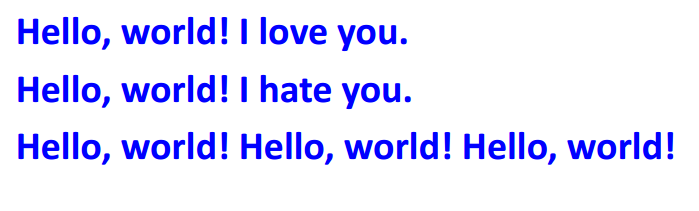
\includegraphics[width=0.5\textwidth]{diagrams/lz77_1.png}\end{figure}
\begin{figure}[H] \caption{Compression starts with literal representation.}
\centering
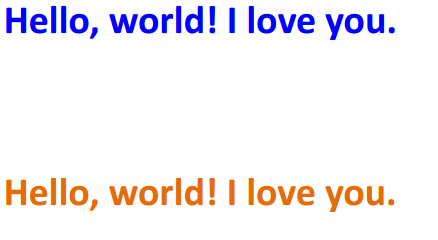
\includegraphics[width=0.35\textwidth]{diagrams/lz77_2.png}\end{figure}
\begin{figure}[H] \caption{We then use a pointer at distance 26 and length 16.}
\centering
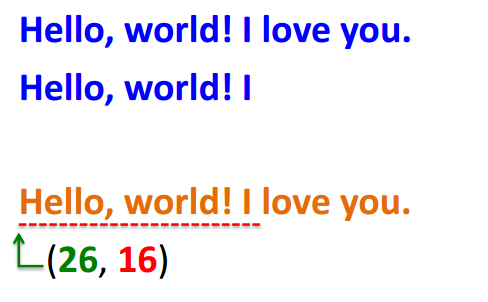
\includegraphics[width=0.35\textwidth]{diagrams/lz77_3.png}\end{figure}
\begin{figure}[H] \caption{We continue with literal.} \centering
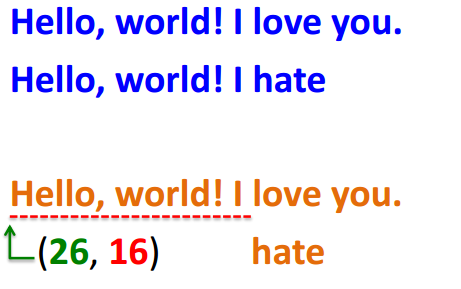
\includegraphics[width=0.35\textwidth]{diagrams/lz77_4.png}\end{figure}
\begin{figure}[H] \caption{We use a pointer pointing to a pointer.} \centering
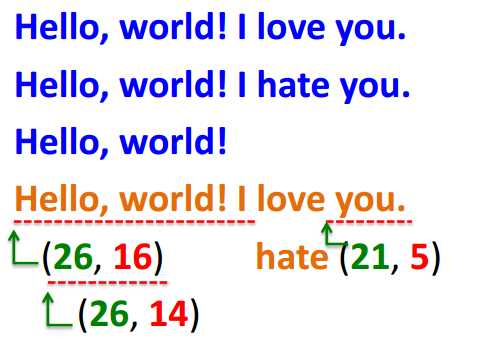
\includegraphics[width=0.35\textwidth]{diagrams/lz77_5.png}\end{figure}
\begin{figure}[H] \caption{We then use a pointer pointing to a pointer pointing
to a pointer.} \centering
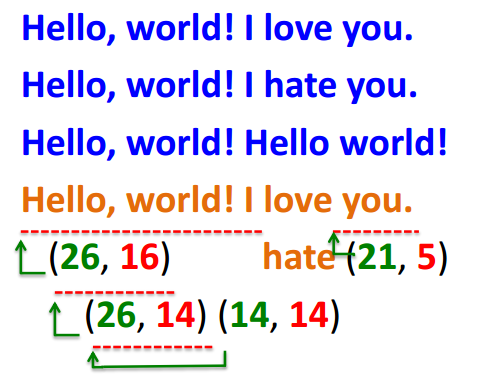
\includegraphics[width=0.35\textwidth]{diagrams/lz77_6.png}\end{figure}
\begin{figure}[H] \caption{Finally, we use a pointer pointing to itself.}
\centering
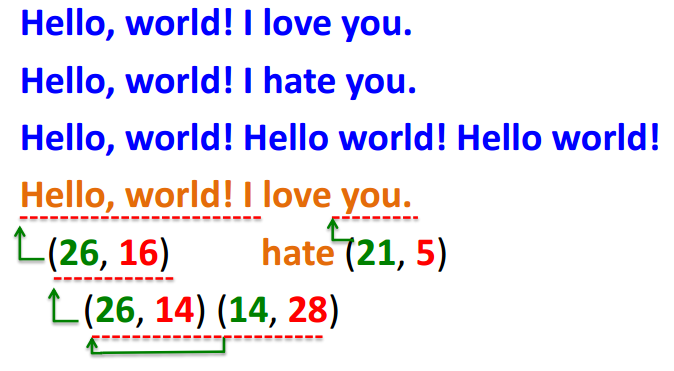
\includegraphics[width=0.5\textwidth]{diagrams/lz77_7.png}\end{figure}


\subsection{Huffman coding}

Huffman coding is also a lossless data compression algorithm developed by David
A. Huffman and published in 1952. \cite{huffman} When compressing a text, a
variable-length code table is created to map source symbols to bitstreams. Each
source symbol can be of less or more bits than originally and the mapping table
is used to translate source symbols into bitstreams during compression and vice
versa during decompression. The mapping table could be represented by a binary
tree of nodes. Each leaf node represents a source symbol, which can be accessed
from the root by following the left path for 0 and the right path for 1. Each
source symbol can be represented only by leaf nodes, therefore the code is
prefix-free, meaning no bitstream representing a source symbol can be the prefix
of any other bitstream representing a different source symbol. The final mapping
of source symbols to bistreams is calculated by finding the frequency of
appearance for each source symbol of the plaintext. That way, most common
symbols can be coded in shorter bitstreams, thus compressing the initial text.

Below follows an example of a plaintext and a valid Huffman tree for compressing
it:

\bigskip \centerline{\textit{\textbf{Chancellor on bring of second bailout for
banks}} \footnote{\url{https://en.bitcoin.it/wiki/Genesis_block}}}

\bigskip \centerline{\textbf{Frequency Analysis}}

\begin{table}[H] \centering \begin{tabular}{ | l | l | l | l | } \hline
\textbf{o}: 6 & \textbf{n}: 5 & \textbf{r}: 3 & \textbf{l}: 3 \\ \textbf{b}: 3 &
\textbf{c}: 3 & \textbf{a}: 3 & \textbf{s}: 2 \\ \textbf{k}: 2 & \textbf{e}: 2 &
\textbf{i}: 2 & \textbf{f}: 2 \\ \textbf{h}: 1 & \textbf{d}: 1 & \textbf{t}: 1 &
\textbf{u}: 1 \\ \hline \end{tabular} \end{table}

\centerline{\textbf{Huffman tree}}

\begin{table}[H] \centering \begin{tabular}{ | l | l | l | l | } \hline
\textbf{o}: 00 & \textbf{n}: 01 & \textbf{r}: 1000 & \textbf{l}: 1001 \\
\textbf{b}: 1010 & \textbf{c}: 1011 & \textbf{a}: 11000 & \textbf{s}: 11001 \\
\textbf{k}: 11010 & \textbf{e}: 11011 & \textbf{i}: 11100 & \textbf{f}: 1111000
\\ \textbf{h}: 1111001 & \textbf{d}: 1111010 & \textbf{t}: 1111011 & \textbf{u}:
1111100 \\ \hline \end{tabular} \end{table}

\centerline{\textbf{Initial text size: 320 bits}} \centerline{\textbf{Compressed
text size: 167 bits}}

\section{Same-origin policy}\label{sec:sameorigin}

Same-origin policy is an important aspect of the web application security model.
According to that policy, a web browser allow scripts contained in one page to
access data in a second page only if both pages have the same \textit{origin}.
Origin is defined as the combination of Uniform Resource Identifier scheme,
hostname and port number. For example, a document retrieved from the website
\textit{http://example.com/target.html} is not allowed under the same-origin
policy to access the Document-Object Model of a document retrieved from
\textit{https://head.example.com/target.html}, since the two websites have
different URI schema (\textit{http} vs \textit{https}) and different hostname
(\textit{example.com} vs \textit{head.example.com}).

Same-origin policy is particularly important in modern web applications, that
rely greatly on HTTP cookies to maintain authenticated sessions. If same-origin
policy was not implemented the data confidentiality and integrity of cookies, as
well as every other content of web pages, would have been compromised. However,
despite the application of same-origin policy by modern browsers, there exist
attacks that enable an adversary to bypass it and breach a user's communication
with a website. Two such major types of vulnerabilities, cross-site scripting
and cross-site request forgery are described in the following subsections.

\subsection{Cross-site scripting}

Cross-site scripting (XSS) is a security vulnerability that allows an adversary
to inject client-side script into web pages viewed by other users. That way,
same-origin policy can be bypassed and sensitive data handled by the vulnerable
website may be compromised. XSS could be divided into two major types,
\textit{non-persistent} and \textit{persistent}
\footnote{\url{https://en.wikipedia.org/wiki/Cross-site_scripting}}, which we
will describe below.

Non-persistent XSS vulnerabilities are the most common. They show up when the
web server does not parse the input in order to escape or reject HTML control
characters, allowing for scripts injected to the input to run unnoticeable.
Usual methods of performing non-persistent XSS include mail or website url links
and search requests.

Persistent XSS occurs when data provided by the attacker are stored by the
server. Responses from the server to different users will then include the
script injected from the attacker, allowing it to run automatically on the
victim's browsers without needing to target them individually. An example of
such attack is when posting texts on social networks or message boards.

\subsection{Cross-site request forgery}

Cross-site request forgery (CSRF) is an exploit that allows an attacker to issue
unauthorized commands to a website, on behalf of a user the website trusts.
Hence the attacker can forge a request to perform actions or post data on a
website the victim is logged in, execute remote code with root privileges or
compromise a root certificate, resulting in a breach of a whole public key
infrastructure (PKI).

CSRF can be performed when the victim is trusted by a website and the attacker
can trick the victim's browser into sending HTTP requests to that website. For
example, when a Alice visits a web page that contains the HTML image tag
\textit{<img
src="\url{http://bank.example.com/withdraw?account=Alice&amount=1000000&for=Mallory}">}
\footnote{\url{https://en.wikipedia.org/wiki/Cross-site_request_forgery}} that
Mallory has injected, a request from Alice's browser to the example bank's
website will be issued, stating for an amount of 1000000 to be transfered from
Alice's account to Mallory's. If Alice is logged in the example bank's website,
the browser will include the cookie containing Alice's authentication
information in the request, making it a valid request for a transfer. If the
website does not perform more sanity checks or further validation from Alice,
the unauthorized transaction will be completed. An attack such as this is very
common on Internet forums that allow users to post images.

A method of mitigation of CSRF is a Cookie-to-Header token. The web application
sets a cookie that contains a random token that validates a specific user
session. Javascript on client side reads that token and includes it in a HTTP
header sent with each request to the web application. Since only Javascript
running within the same origin will be allowed to read the token, we can assume
that it's value is safe from unauthorized scripts to read and copy it to a
custom header in order to mark a rogue request as valid.

\section{Transport Layer Security}\label{sec:tls}

Transport Layer Security (TLS) is a protocol that provides communications
security over the internet, allowing a server and a client to communicate in a
way that prevents eavesdropping, tampering or message forgery. \cite{tls12}

The users negotiate a symmetric key via assymetric cryptography that is provided
by X.509 certificates, therefore there exist certificate authorities and a
public key infrastructure (PKI), in order for the certificates to be verified
for their owners. However, it can be understood that, due to their key role,
certificate authorities are points of failure in the system, enabling for
Man-in-the-Middle attacks, in a case when an adversary has managed to forge
a root certificate.

Apart from certificate-related attacks, a well-known category is compression
attacks. \footnote{\url{https://tools.ietf.org/html/rfc7457}} Such attacks
exploit TLS-level compression so as to decrypt ciphertext. In this document, we
investigate the threat model and performance of such an attack,
\href{http://breachattack.com}{BREACH}.

In the following subsections we will briefly describe some of the protocol
details, especially handshake and the format of TLS records.

\subsection{TLS handshake}

\begin{figure}[H] \caption{TLS handshake flow.} \centering
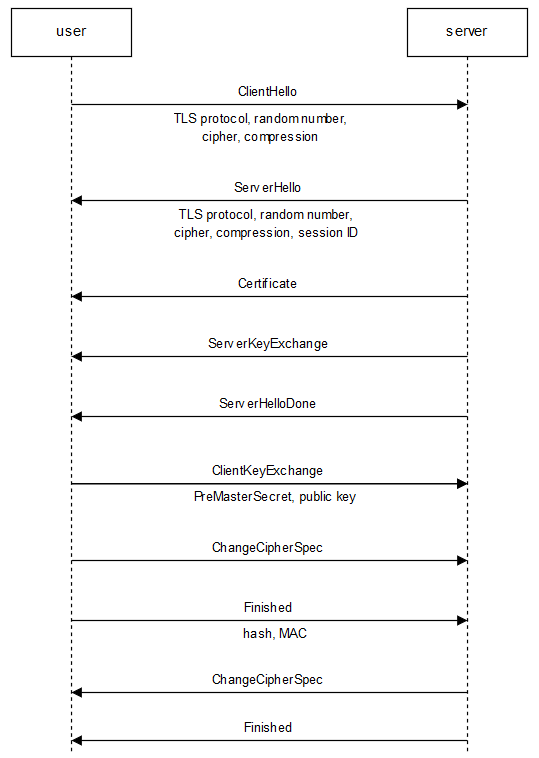
\includegraphics[width=0.7\textwidth]{diagrams/tls_handshake.png}\end{figure}

This sequence diagram presents the functionality of TLS handshake. User and
server exchange the basic parameters of the connection, specifically the
protocol version, cipher suite, compression method and random numbers, with the
ClientHello and ServerHello records. The server then provides all information
needed from the user to validate and use the asymmetric server key, in order to
compute the symmetric key to be used in the rest of the communication. The
client computes a \textit{PreMasterKey}, that is sent to the server, which is
used by both parties to compute the symmetric key. Finally, both sides exchange
and validate hash and MAC over the previous messages, after which they both have
the ability to communicate safely.

The above flow describes the basic TLS handshake. Client-authenticated and
resumed handshakes have similar functionality, which are not relevant for the
purpose of this paper.

\subsection{TLS record}

\begin{figure}[H] \caption{TLS record.} \centering
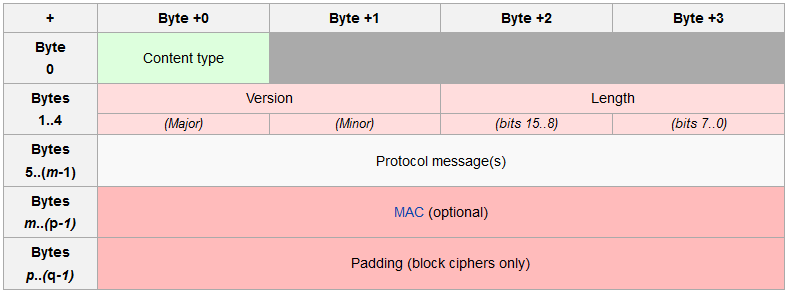
\includegraphics[width=1\textwidth]{diagrams/tls_record.png}\end{figure}

The above figure
\footnote{\url{https://en.wikipedia.org/wiki/Transport_Layer_Security}} depicts
the general format of all TLS records.

The first field describes the Record Layer Protocol Type contained in the
record, which can be one of the following:

\begin{table}[H] \centering \begin{tabular}{ | l | l | } \hline \textbf{Hex} &
\textbf{Type} \\ \hline 0x14 & ChangeCipherSpec \\ 0x15 & Alert \\ 0x16 &
Handshake \\ 0x17 & Appliation \\ 0x18 & Heartbeat \\ \hline \end{tabular}
\end{table}

The second field defines the TLS version for the record message, which is
identified my the major and minor version as below:

\begin{table}[H] \centering \begin{tabular}{ | l | l | l | } \hline
\textbf{Major} & \textbf{Minor} & \textbf{Version} \\ \hline 3 & 0 & SSL 3.0 \\
3 & 1 & TLS 1.0 \\ 3 & 2 & TLS 1.1 \\ 3 & 3 & TLS 1.2 \\ \hline \end{tabular}
\end{table}

The length of the contained record message, MAC and padding is then calculated
by the following two fiels as: \begin{math}256*(bits 15..8) + (bits
7..0)\end{math}.

Finally, the payload of the record, which, depending on the type, may be
encrypted, the MAC, if provided, and the padding, if needed, make up the rest of
the TLS record.

\section{Man-in-the-Middle}\label{sec:mitm}

Man-in-the-Middle (MitM) is one of the most common attack vectors, where an
attacker reroutes the communication of two parties, in order to be controlled
and possibly altered. The aggressiveness of the attack can vary from passive
eavesdropping to full control of the communication, as long as the attacker is
able to impersonate both parties and convince them to be trusted.

\begin{figure}[H] \caption{Man-in-the-Middle.} \centering
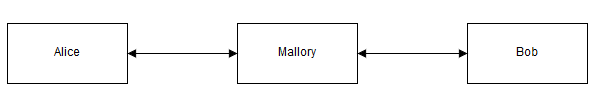
\includegraphics[width=1\textwidth]{diagrams/mitm.png}\end{figure}

MitM attacks can be mitigated by using end-to-end cryptography, mutual
authentication or PKIs. However, some attacks manage to bypass such mitigation
techniques. Below, we descripe two such attacks, ARP Spoofing and DNS cache
poisoning.

\subsection{ARP Spoofing} ARP spoofing

\footnote{\url{https://en.wikipedia.org/wiki/ARP_spoofing}} is a technique where
an attacker sends Address Resolution Protocol (ARP) messages over the network,
so as to assosiate the MAC address with the IP address of another host. That
way, the attacker may intercept the traffic of the network, modify or deny
packets, performing denial of service, MitM or session hijacking attacks.

\begin{figure}[H] \caption{Arp Spoofing.} \centering
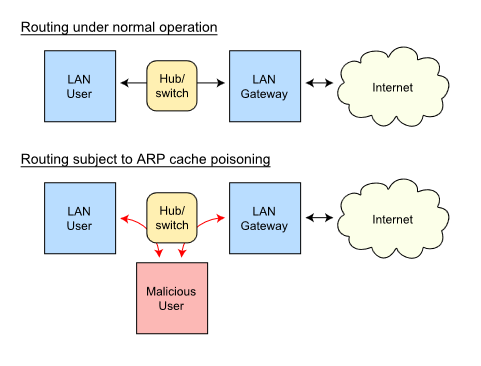
\includegraphics[width=0.8\textwidth]{diagrams/arp_spoofing.png}\end{figure}

ARP spoofing can be also used for legitimate reasons, when a developer needs to
debug IP traffic between two hosts. That way, the developer can act as proxy
between the two hosts or configure the switch that is normally used by the two
parties to forward traffic for monitoring.

\subsection{DNS spoofing}

\begin{figure}[H] \caption{DNS Spoofing.} \centering
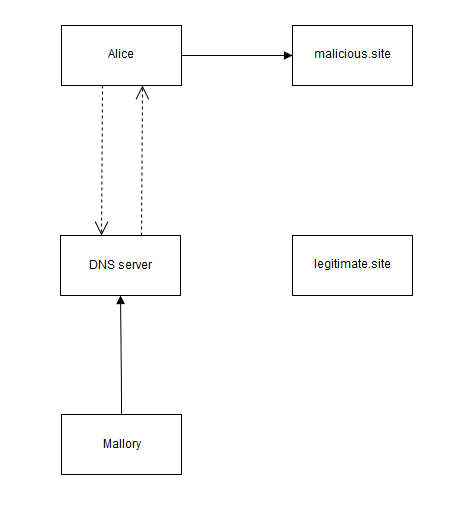
\includegraphics[width=0.5\textwidth]{diagrams/dns_spoofing.png}\end{figure}

DNS spoofing (or DNS cache poisoning) is an attack, when the adversary
introduces data into a Domain Name System resolver's cache, in order to return
an incorrect address for a specific host.

DNS servers are usually provided by Internet Service Providers (ISPs), used to
resolve IP addresses to human-readable hostnames faster. A malicious employee,
or anyone that has gained unauthorized access to the server, can then perform
DNS poisoning, affecting every user that is being serviced by that server.

\chapter{Partially Chosen Plaintext Attack}\label{ch:pcpa}

Traditionally, cryptographers have used games for security analysis. Such games
include the indistinguishability under chosen-plaintext-attack (IND-CPA), the
indistinguishability under chosen ciphertext attack/adaptive chosen ciphertext
attack (IND-CCA1, IND-CCA2) etc
\footnote{\url{https://en.wikipedia.org/wiki/Ciphertext_indistinguishability}}.
In this chapter, we introduce a definition for a new property of encryption
schemes, called indistinguishability under partially-chosen-plaintext-attack
(IND-PCPA). We will also show provide comparison between IND-PCPA and other
kwown forms of cryptosystem properties.

\section{Partially Chosen Plaintext Indistinguishability}\label{sec:indpcpa}

\subsection{Definition} IND-PCPA uses a definition similar to that of IND-CPA.
For a probabilistic asymmetric key encryption algorithm, indistinguishability
under partially chosen plaintext attack (IND-PCPA) is defined by the following
game between an adversary and a challenger.

\begin{itemize} \item The challenger generates a pair \begin{math}P_k,
S_k\end{math} and publishes \begin{math}P_k\end{math} to the adversary.  \item
The adversary may perform a polynomially bounded number of encryptions or other
operations.  \item Eventually, the adversary submits two distinct chosen
plaintexts \begin{math}M_0, M_1\end{math} to the challenger.  \item The
challenger selects a bit \begin{math}b\in{0, 1}\end{math} uniformly at random.
\item The adversary can then submit any number of selected plaintexts
\begin{math}R_i, i\in N, |R| \geq 0\end{math}, so the challenger sends the
ciphertext \begin{math}C_i = E(P_k, M_b||R_i)\end{math} back to the adversary.
\item The adversary is free to perform any number of additional computations or
encryptions, before finally guessing the value of \begin{math}b\end{math}.
\end{itemize}

A cryptosystem is indistinguishable under partially chosen plaintext attack, if
every probabilistic polynomial time adversary has only a negligible advantage on
finding \begin{math}b\end{math} over random guessing. An adversary is said to
have a negligible advantage if it wins the above game with probability
\begin{math}\frac{1}{2} + \epsilon(k)\end{math}, where
\begin{math}\epsilon(k)\end{math} is a negligible function in the security
parameter \begin{math}k\end{math}.

Intuitively, we can think that the adversary has the ability to modify the
plaintext of a message, by appending a portion of data of his own choice to it,
without knowledge of the plaintext itself. He can then acquire the ciphertext of
the modified text and perform any kinds of computations on it. A system could
then be described as IND-PCPA, if the adversary is unable to gain more
information about the plaintext, than he could by guessing at random.

\subsection{IND-PCPA vs IND-CPA}

Suppose the adversary submits the empty string as the chosen plaintext, a choice
which is allowed by the definition of the game. The challenger would then send
back the ciphertext \begin{math}C_i = E(P_k, M_b||"\ ") = E(P_k, M_b)\end{math},
which is the ciphertext returned from the challenger during the IND-CPA game.
Therefore, if the adversary has the ability to beat the game of IND-PCPA, i.e. if
the system is not indistinguishable under partially chosen plaintext attacks, he
also has the ability to beat the game of IND-CPA. Thus we have shown that
IND-PCPA is at least as strong as IND-CPA.

\section{PCPA on compressed encrypted protocols}\label{sec:cepcpa}

\subsection{Compression-before-encryption and vice versa} When having a system
that applies both compression and encryption on a given plaintext, it would be
interesting to investigate the order the transformations should be executed.

Lossless data compression algorithms rely on statistical patters to reduce the
size of the data to be compressed, without losing information. Such a method is
possible, since most real-world data has statistical redundancy. However, it can
be understood from the above that such compression algorithms will fail to
compress some data sets, if there is no statistical pattern to exploit.

Encryption algorithms rely on adding entropy on the ciphertext produced. If the
ciphertext contains repeated portions or statistical patterns, such behaviour
can be exploited to deduce the plaintext.

In the case that we apply compression after encryption, the text to be
compressed should demostrate no statistical analysis exploits, as described
above. That way compression will be unable to reduce the size of the data. In
addition, compression after encryption does not increase the security of the
protocol.

On the other hand, applying encryption after compression seems a better
solution. The compression algorithm can exploit the statistical redundancies of
the plaintext, while the encryption algorithm, if applied perfectly on the
compressed text, should produce a random stream of data. Also, since compression
also adds entropy, this scheme should make it harder for attackers who rely on
differential cryptanalysis to break the system.

\subsection{PCPA scenario on compression-before-encryption protocol}

Let's assume a system that composes encryption and compression in the following
manner:

\begin{math}c = Encrypt(Compress(m))\end{math}

where \begin{math}c\end{math} is the ciphertext and \begin{math}m\end{math} is
the plaintext.

Suppose the plaintext contains a specific secret, among random strings of data,
and the attacker can issue a PCPA with a chosen plaintext, which we will call
reflection. The plaintext then takes the form:

\begin{math}m = n_1 || secret || n_2 || reflection || n_3\end{math}

where \begin{math}n_1, n_2, n_3\end{math} are random nonces.

If the reflection is equal to the secret, the compression mechanism will
recognize the pattern and compress the two portions. In other case, the two
strings will not demonstrate any statistical redundancy and compression will
perform worse. As a result, in the first case the data to be encrypted will be
smaller than in the second case.

Most commonly encryption is done by a stream or a block cipher. In the first
case, the lengths of a plaintext and the corresponding ciphertext are identical,
whereas in the second case they differ by the number of the padding bits, which
is relatively small. That way, in the above case, an adversary could identify a
pattern and extract information about the plaintext, based on the lengths of the
two ciphertexts.

\chapter{Attack Model}\label{ch:attack}

In this chapter, we will extensively present the threat model of BREACH. We will
explain the conditions that should be met in order for the attack to be
launched and describe our implementation for the attack. We will also
investigate the types of vulnerabilities in web applications that can be
exploited with this attack, as well as introduce alternative types of exploits
that have not been presented before.

\section{Mode of Operation}\label{sec:mo}

This section provides the model of the attack, the conditions that are required
for the attack to launch and the implementation that was developed for the
purpose of this paper.

\subsection{Description}

The first step is for the attacker to gain control of the victim's network.
Specifically, the attacker needs to be able to view the victim's encrypted
traffic, which can be accomplished using the Man-in-the-Middle techniques
described in Section \ref{sec:mitm}.

After that, the script that issues the requests needs to be executed from the
victim's browser. One way to do this is to persuade the victim to visit a
website controlled by the attacker. This is usually possible with social
engineering methods.

The script issues multiple requests on the target endpoint which are sniffed by
the attacker. As described in Section \ref{sec:sameorigin}, the attacker cannot
read the plaintext of a response, although the lengths of both the request and
the response is visible on the network.

Each request contains a chosen stream of data that gets reflected in the
response. Since the victim is logged in the targeted endpoint website, the
response body will also contain the secrets. If the conditions defined in
Section \ref{subsec:lz77} are met, the secret and the reflection will be
compressed and encrypted.

By issuing a large amount of requests for different inputs the attacker can
analyse the response lengths and extract information about the secrets when a
response presents different length behaviour than the rest.

\subsection{Man-in-the-Middle implementation}

In order to gain control of the victim's traffic toward a chosen endpoint, we
created a Python script that acts as a Man-in-the-Middle proxy.

The IPs and ports of the victim and the endpoint are configured in the
constants' file and the Python script opens connections over TCP sockets on
both directions so that traffic from the victim to the endpoint and vice versa
is routed through the Man-in-the-Middle proxy.

After the environment is set, the script waits for a packet to be received on
either of the sockets, at which point the source of the packet is identified and
the data is parsed in order to log the TLS header and the payload. Eventually,
the packet is forwarded to the appropriate destination.

The parsing of the packet data is essential, since the header contains
information regarding the version of TLS used as well as the length of the
record.

Trying to spot a fragmented record payload, the length of the packet payload is
compared to the length defined in the TLS header. In case the packet is smaller
than the length declared in the header, the number of remaining bytes is stored,
so that these bytes will be taken into account when following packets of same
origin are received. In case the TLS header is fragmented, which can be deduced
when the total bytes of the packet are less than 5, the actual data fragment
needs to be stored so that, combined with the following packet, it can be
translated to a valid TLS record.

Finally, a TLS downgrade attack mechanism is also implemented. In order to test
whether a TLS downgrade attack is feasible, the \texttt{client hello} packet is
intercepted and dropped while the mitm sends a fatal \texttt{handshake failure}
alert response to the victim. The victim's browser is usually configured to
attempt a connection with a lower TLS version where it should also include the
\texttt{tls\_fallback\_scsv} option in the cipher suite list. If the server is
configured properly, the downgrade attempt should be recognised by the
\texttt{tls\_fallback\_scsv} pseudo-cipher and the connection should be dropped.
In other case, the TLS version could be downgraded to a point where a less safe
connection is established such as SSL 3.0 or using the RC4 stream cipher.

A log from a downgrade attempt against Facebook touch, that was created by our
MitM proxy, can be found in Appendix section \ref{sec:downgrade_log}. For
further information on the downgrade vulnerability see the POODLE attack
\cite{poodle}.

The code of the Man-in-the-Middle proxy, as well as the constants' file, can
be found in Appendix sections \ref{sec:connect_py} and \ref{sec:constants_py}.

\subsection{BREACH Javascript implementation}

For the implementation of the BREACH Javascript, we assume the user has provided
the alphabet that the characters of the secret belong to as well as the known
prefix needed to bootstrap the attack. This information will be written to a
file used by the script that performs the attack, an example of which is shown
below:

\plaintext{file with request parameters.}{serial_request.txt}

The script uses the jquery
library\footnote{\url{http://code.jquery.com/jquery-2.1.4.min.js}} to read the
information from the file and issue the attack. If the file is corrupt or either
of the attack variables has changed, a delay of 10 seconds is introduced, until
the system is balanced. After that, serial requests for each item of the attack
vector are made, continuing from the beginning when the end of the vector is
reached.

A delay of 10 seconds is also introduced if the above function fails for any
reason, i.e. if the information file does not exist. That way the attack is
persistent and it is the framework's responsibility to provide the script with a
valid information parameters' file.

For the purpose of this paper, the script was included in a local minimal HTML
web page that was visited in order for the attack to begin. However, with slight
modifications it could be run on real world applications or be injected in HTTP
responses, as described in the following section.

The BREACH script and the HTML web page can be found in the Appendix sections
\ref{sec:evil_js} and \ref{sec:index_html}.

\subsection{Attack persistence}\label{sec:persistence}

In this section we will propose a \texttt{command-and-control} mechanism that
makes the attack much more practical. Specifically, we will describe how the
attack can be implemented even if the victim does not visit a contaminated web
page but simply browses the HTTP web.

Since the attacker controls the victim's network, it is possible to inject the
attack script in a response from a regular HTTP website. The script will then
run on the victim's browser, as if the script was part of the HTTP web page all
along.

The following figure depicts this methodology, which is based on the fact that
regular HTTP traffic is not encrypted and also does not ensure data integrity.

\begin{figure}[h] \caption{command-and-control mechanism.} \centering
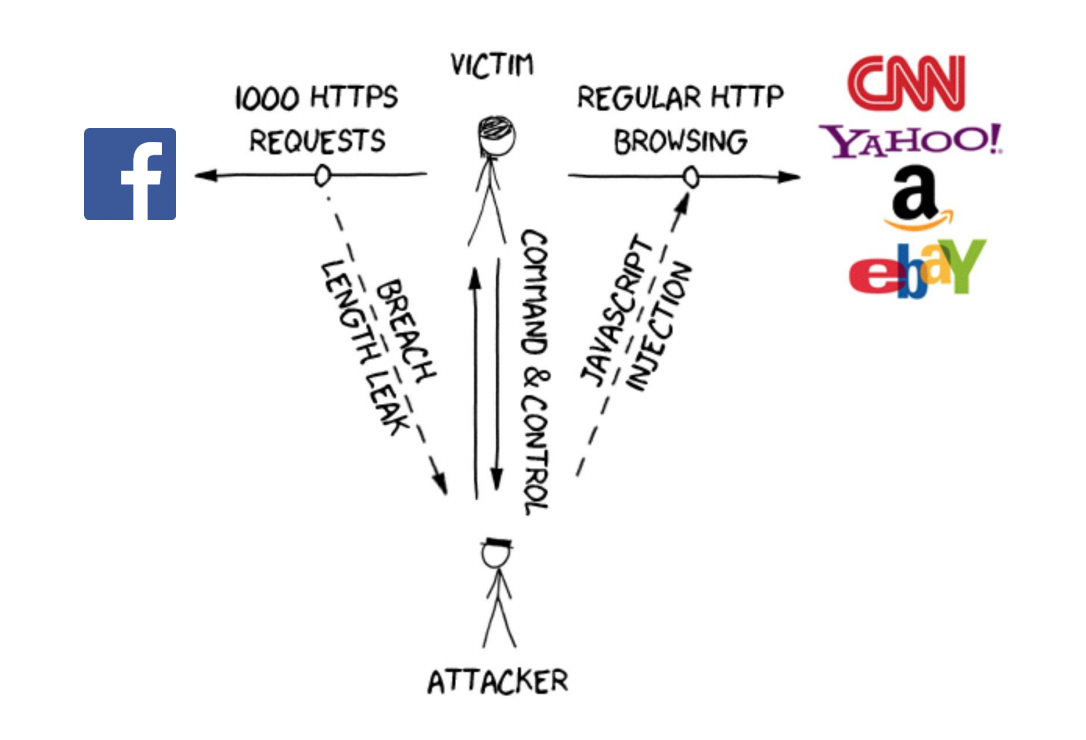
\includegraphics[width=0.6\textwidth]{diagrams/breach_mitm.png}\end{figure}

It is clear that even if the victim stops the connection with the specific HTTP
website, the script can be injected in the next HTTP website that is requested,
resuming the attack session from where it was stopped.

\section{Vulnerable endpoints}\label{sec:vulnerabilities}

In the original BREACH paper \cite{breach}, Gluck, Harris and Prado investigated
the use of CSRF tokens included in HTTP responses as secrets to be stolen.
In this paper we suggest alternative secrets as well as point out specific
vulnerabilities on widely used web applications, such as Facebook and Gmail.

\subsection{Facebook Chat messages}\label{subsec:fb}

Facebook is the biggest social network as of 2015 with millions of people using
its chat functionality to communicate. The mobile version, Facebook
Touch\footnote{\url{https://touch.facebook.com}} provides a lightweight
alternative for faster browsing. In this paper we present a vulnerability
that allows an attacker to steal chat messages from Facebook Touch, using the
BREACH attack.

Mobile versions of websites provide a good alternative compated to full versions
for a list of reasons. Firstly, these endpoints provide limited noise, given
that they provide a lighter user interface compared to full versions.  Noise
can be defined as any kind of string that changes between requests, such as
timestamps or tokens, which consequently affects the length of the
compressed HTML code even for the same request URL. Secondly, given that the
plaintext is smaller in mobile versions, the possibility of the text that
exists between the secret and the reflection to be larger than the window of
the LZ77 compression is reduced.

Facebook has launched a mechanism to prevent the original BREACH attack against
CSRF
tokens\footnote{\url{https://www.facebook.com/notes/protect-the-graph/preventing-a-breach-attack/1455331811373632?_rdr=p}}.
However, as of August 2015, it has not created a mitigation technique against
the same attack on private messages. An attack method that could steal such
messages is described in the following paragraphs.

Facebook Touch provides a search functionality via URL, where one can search for
messages or friends. Specifically, when a request is made for
\url{https://touch.facebook.com/messages?q=}<search\_string>, the response
contains the chat search results for the given search string. If no match is
found, the response consists of an empty search result page. However, this page
also contains the last message of the 5 latest conversations, which can be seen
in the top drop-down message button of the Facebook user interface, as depicted
below:

\begin{figure}[h] \caption{Facebook Chat drop-down list.} \centering
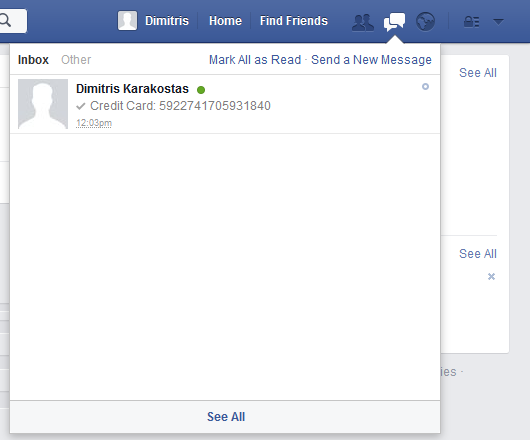
\includegraphics[width=0.6\textwidth]{diagrams/fb_message.png}\end{figure}

The next step is to validate that the search string is reflected in the
response, which should also contain the private secret. Below is a fragment of
the HTML response body, where it can be clearly seen that this condition is met:

\begin{figure}[h] \caption{Facebook response body containing both secret and
reflection.} \centering
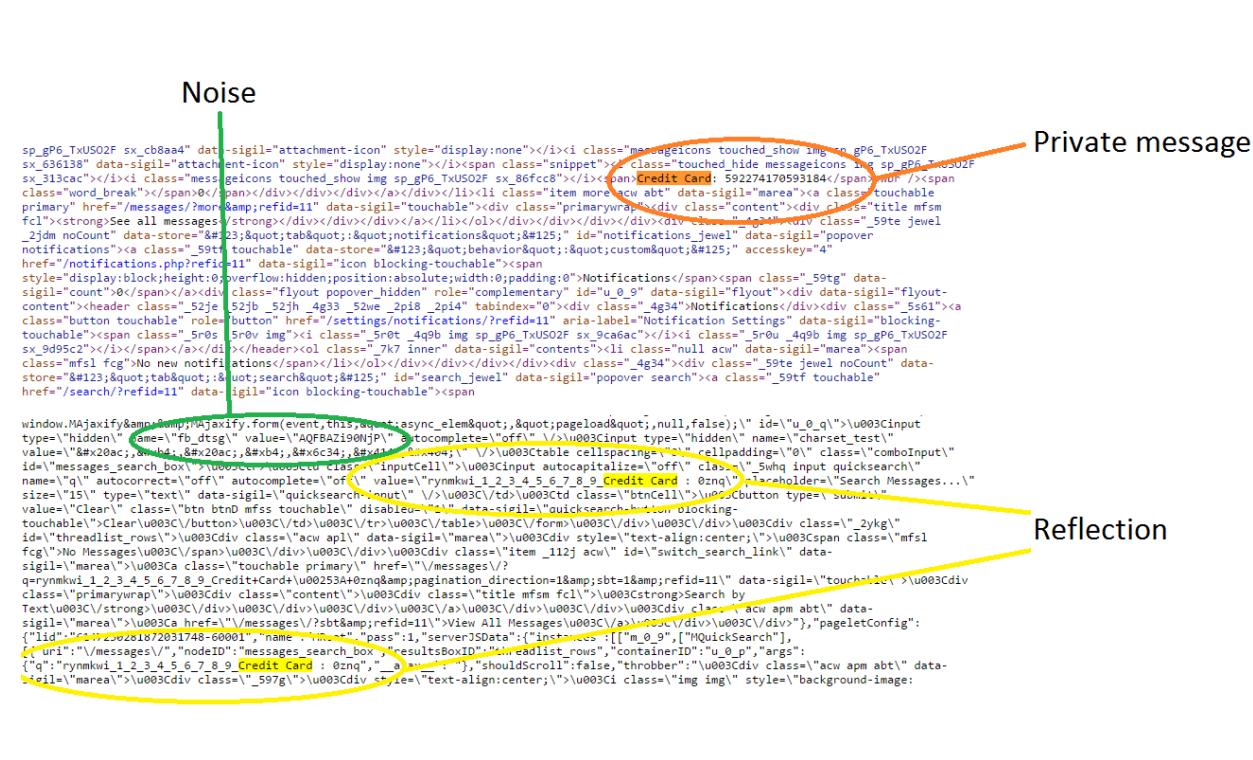
\includegraphics[width=1.1\textwidth]{diagrams/fb_response.png}\end{figure}

If the search string was not reflected in the response the attack could still
be feasible, as long as the attacker could send private messages to the victim.
In that case the private messages from the attacker would be included in the
latest conversations list along with the secret messages from third friends of
the victim, resulting in the compression between the two and thus the partially
chosen plaintext attack.

So, at this point, one of the basic assumptions of the attack, the fact that a
secret and an attacker input string should both be contained in the response,
has been confirmed, providing us with a vulnerability that can be exploited in
the context of the attack.

\subsection{Gmail authentication token}\label{subsec:gmail_token}

Gmail is one of the most used and trusted mail clients as of 2015. It also
provides a plain HTML version for faster, lightweight
interaction\footnote{\url{https://m.gmail.com}}. Gmail uses an authentication
token, which is a random string of digits, letters (uppercase and lowercase) and
dashes, generated every time the user logs in the account.

Opposed to Facebook, Google has not issued any mechanism to mask the
authentication token for different user sessions, but instead uses the same
token for a large amount of requests. This functionality could possibly result
to a threat against the confidentiality of the account.

Requests on \url{m.gmail.com} redirect to another directory of the full website,
specifically \url{https://mail.google.com/mail/u/0/x/}<random\_string>, where
the random string is generated for every request and can be used only for the
particular session.

Gmail also provides a search via URL functionality, similar to the one described
for Facebook Touch. Specifically, a user can search for mails using a URL such
as \url{https://mail.google.com/mail/u/0/x/?s=q&q=}<search\_string>. If no
valid string is provided in the place where the random string is supposed
to be, Google will redirect the request to a URL where the vacation will be
filled with a randomly generated string and return an empty result page,
stating the search action as incomplete, as shown below:

\begin{figure}[h] \caption{Invalid Gmail search.} \centering
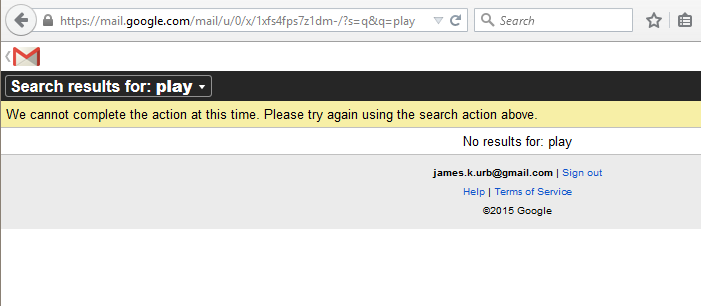
\includegraphics[width=1\textwidth]{diagrams/gmail_search.png}\end{figure}

However, the HTML body of the response contains both the search string and the
authentication token, as can be seen in the following figure:

\begin{figure}[h] \caption{Gmail response body containing both secret and
reflection.} \centering
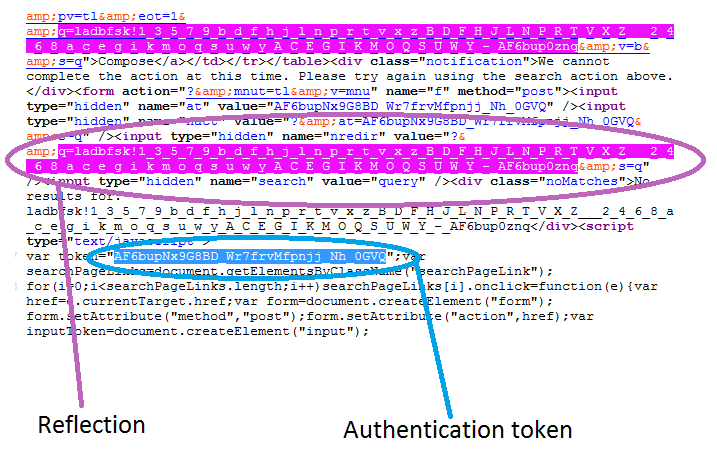
\includegraphics[width=1\textwidth]{diagrams/gmail_response.png}\end{figure}

Another vulnerability that can be exploited is when trying to find the first
three characters to bootstrap the attack. In the response body, the
authentication token is included as below:

\begin{figure}[h] \caption{Gmail authentication token.} \centering
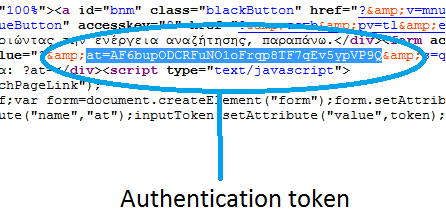
\includegraphics[width=0.6\textwidth]{diagrams/gmail_bootstrap.png}\end{figure}

The authentication token is preceded by the characters \texttt{at=}, which can
be used as the initiating prefix of the attack. Furthermore, the prefix
\texttt{AF6bup} of the token is static, regardless of the session and the
account used. This prefix can also be used in a similar manner to bootstrap the
attack.

\subsection{Gmail private emails}\label{subsec:gmail_mail}

Another opportunity for attack is provided by the search functionality of the
full gmail website. If a user issues a search request in a URL like
\url{https://mail.google.com/mail/u/0#search/}<search\_string> and the search
response is empty, the HTML body will also contain both the subject and an
initial fragment of the body of the latest inbox mails:

\begin{figure}[h] \caption{Gmail empty search response containing latest mails.}
\centering
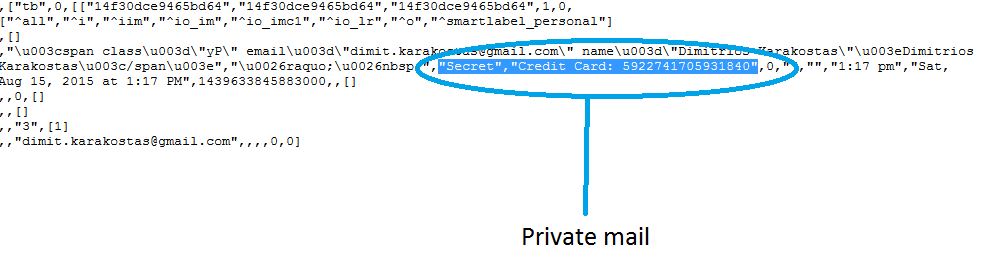
\includegraphics[width=1.1\textwidth]{diagrams/gmail_plain_response.png}\end{figure}

Although in that case the response body does not include the search string, an
attacker could send multiple mails to the victim, which would be included in the
response along with other new messages. That way the attacker could insert a
chosen plaintext in the HTML body and configure the attack under that context.

The above vulnerability shows that secrets and attacker input cannot always be
distinguished. In this case both the secret and the input are emails
making the mitigation of the attack particularly hard.

\section{Validation of secret-reflection compression}\label{sec:mitmproxy}

In previous sections, we have found multiple vulnerabilities on known websites.
We have confirmed that the attacker's chosen plaintext and the secret are both
contained in the HTML response body. In this section, we will present a
methodology to confirm that the chosen plaintext and the secret are also
compressed well when the plaintext matches the secret and badly in any other
case.

The first tool used is mitmproxy\footnote{\url{https://mitmproxy.org}}.
Mitmproxy is described as "an interactive console program that allows traffic
flows to be intercepted, inspected, modified and replayed". For the purposes of
our work, mitmproxy was used to extract the compressed HTML body of two search
request, in the Facebook context described in section \ref{subsec:fb}. The first
search string contained a selected prefix followed by an incorrect character,
while the second contained the same prefix followed by the correct character of
the secret.

The second tool used is infgen\footnote{\url{http://www.zlib.net/infgen.c.gz}}.
infgen is a disassembler that gets a gzip stream as input and outputs the
Huffman tables and the LZ77 compression of the initial data stream.

Applying infgen on the two HTML responses we obtained with mitmproxy, the
comparison between the correct and the incorrect search string can be seen in
the following figure:

\begin{figure}[h] \caption{Comparison of two compressed responses.}
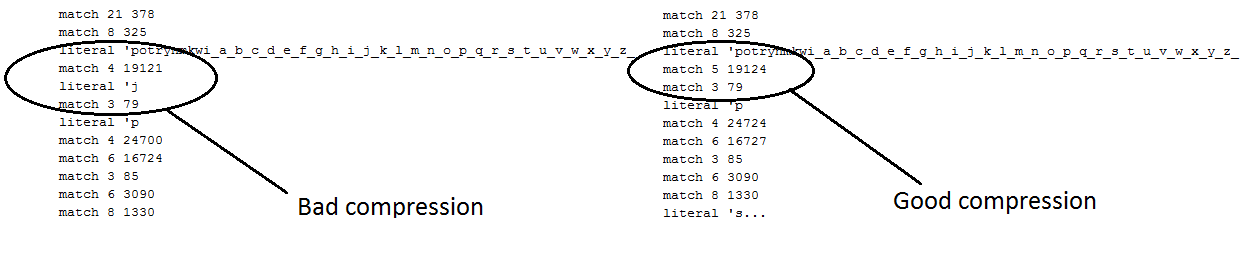
\includegraphics[width=1.15\textwidth]{diagrams/compression_comparison.png}\end{figure}

The left part of the figure shows the compression when the incorrect character
is used. In that case, the prefix is matched so 4 characters are compressed,
while the next character is not compressed and is included as a literal instead.

The right part shows the correct character compression, in which case both the
prefix and the character are compressed, resulting in 5 total characters to be
included in the reference statement and no literal statement.

It is understood that in the second case, since the compression is better the
LZ77 compressed text is smaller, possibly resulting to the final encrypted text
being smaller.

The above described methodology can be used in general in order to test whether
a website compresses two portions of text and to verify that the conditions of a
PCPA attack are met.

\chapter{Statistical methods}\label{ch:statistic}

Gluck, Harris and Prado in the original BREACH paper investigated the attack
on stream ciphers such as RC4. They also suggested that block ciphers are
vulnerable without providing practical attack details. However, the use of RC4
is prohibited in negotiation between servers and clients
\cite{rc4_prohibit} due to several other major vulnerabilities.

In this work we perform practical attacks against popular block ciphers by
using statistical methods to by-pass noise created from random portions of data
stream, padding or the Huffman coding. Also we propose various optimization
techniques that can make the attack much more efficient.

\section{Probabilistic techniques}\label{sec:probabilistic}

Block ciphers provide a greater challenge compared to stream ciphers when it
comes to telling length apart, since stream ciphers provide better granularity.
In this work we use statistical techniques to overcome this problem.

Furthermore, Huffman coding may affect the length of the compressed data stream,
since the character frequency might be affected resulting to different Huffman
tables and subsequently different length. We will propose a method to bypass
Huffman induced noise too.

\subsection{Attack on block ciphers}

Block ciphers are the most common used ciphers in modern websites. Especially
AES \cite{aes} is used in major websites such as
Facebook\footnote{\url{https://www.facebook.com}},
Google\footnote{\url{https://www.google.com}},
Twitter\footnote{\url{https://www.twitter.com}},
Wikipedia\footnote{\url{https://www.wikipedia.org}},
YouTube\footnote{\url{https://www.youtube.com}},
Amazon\footnote{\url{https://www.amazon.com}} and others. In this work we
introduce methods to attack block ciphers using the attack model described in
Chapter \ref{ch:attack}.

First of all, a packet stream of a specific endpoint needs to be examined, in
order to find patterns and better understand the distribution of the data stream
on TLS records and TCP packets. In the following figures request streams can be
seen for Facebook Touch and Gmail respectively.

\begin{figure}[H] \caption{Facebook flow} \centering
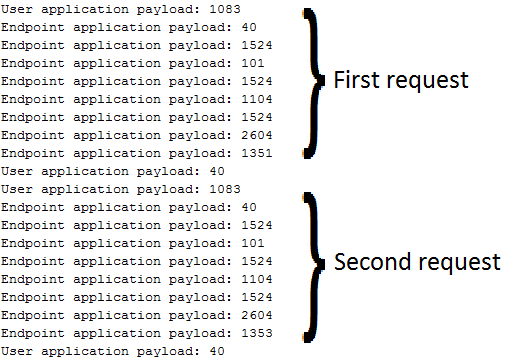
\includegraphics[width=0.6\textwidth]{diagrams/facebook_request_flow.png}\end{figure}

\begin{figure}[H] \caption{Gmail flow} \centering
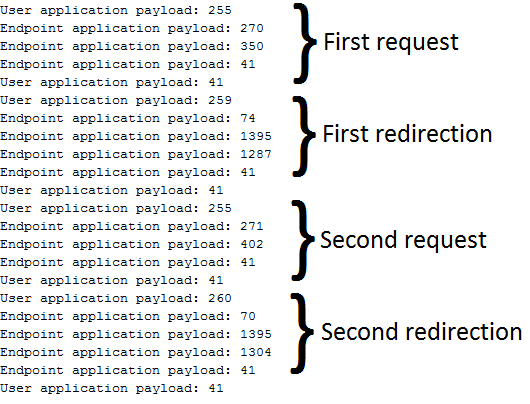
\includegraphics[width=0.6\textwidth]{diagrams/gmail_request_flow.png}\end{figure}

A close look on the above record stream reveals interesting information about
the pattern presented by multiple requests on the same endpoint.

Specifically the first figure shows two consequent requests on the search
method of Facebook Touch. The two requests were issued under the attack context
and it can be seen that their lengths differ only in a single TLS record.

At this point it would be safe to assume that the specific record that differs
in the two requests is the one containing the attacker's chosen plaintext. In
order to confirm this, mitmproxy can again be used along with the MitM proxy we
have developed.

Mitmproxy uses netlib\footnote{\url{https://pypi.python.org/pypi/netlib}} as a
data-link library. Netlib's \texttt{read\_chunked} function performs the reading
of the TLS record fragments. We added \texttt{print} markers in this function,
which mark the log that contains the packet flow passing through our MitM proxy
and also provides the sectors that the plaintext is divided before compression.
Comparing the log with the decrypted and decompressed chunks of plaintext we
have confirmed that the sector of the plaintext that contains the reflection is
contained in the TLS record that differs in the length flow.

The above flows lead to another interesting deduction. If the implementation of
the block cipher was as expected, each record should have been of length that is
a product of 128 bits and consequently the two records that differ should have
had the same length or differ on a product of 128 bits. However, that is
not the case here.

In order to further investigate the implementation of block ciphers, we have
issued the attack on multiple operating systems, networks and browsers. The
parameter that seemed to demonstrate similar behaviour on these cases was the
browser, as for different OSs and networks the packet flow was structurally the
same for the same browser version.

In the following figures we present two distinct packet flow structures that
were observed during the experiments on different browsers and versions.

\begin{figure}[H] \caption{Older browser version} \centering
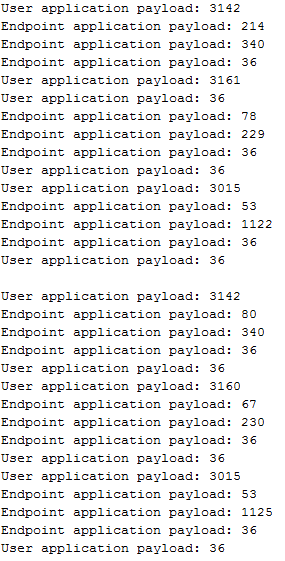
\includegraphics[width=0.4\textwidth]{diagrams/older_browser_version.png}\end{figure}

\begin{figure}[H] \caption{Newer browser version} \centering
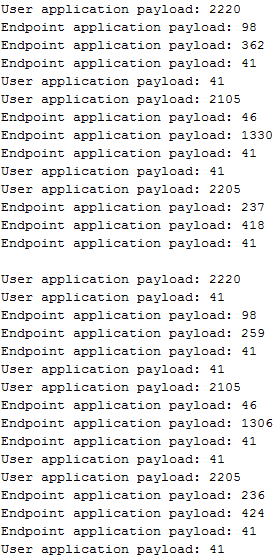
\includegraphics[width=0.4\textwidth]{diagrams/newer_browser_version.png}\end{figure}

In older browser versions, the packet that contains the reflection is the one
with length 1122 for the first request and 1125 for the second request. Each
request of the flow demonstrated a difference of a few bytes, that would not
exceed 20 at any time. In newer versions of browsers, the packet that contains
the reflection 418 bytes for the first request and 424 for the second. In other
cases the difference could be tens or hundreds of bytes for two requests.

The browsers that were used, Mozilla Firefox, Google Chrome, Chromium and Iceweasel,
all use Mozilla's Network Security Services (NSS)
library\footnote{\url{https://developer.mozilla.org/en-US/docs/Mozilla/Projects/NSS}}
for the implementation of TLS. Following the above discoveries, we have found
that the first pattern was demonstrated in browser versions that used NSS
3.17.3 release or older, whereas the second pattern was demonstrated on browsers
that used newer NSS releases. However, further investigation needs to be done,
in order to determine why the block cipher implementation does not follow the
theoretical standards.

In any case, the above patterns allow us to use statistical methods to extract
conclusions regarding the length. Specifically by issuing hundreds or thousands
of requests for the same string and calculating the mean length of the
responses the correct symbol should converge in a smaller mean length that an
incorrect. This method also allows us to bypass noise introduced by random
strings in the HTML body.

\subsection{Huffman fixed-point}

Huffman coding, as described in Section \ref{subsec:huffman}, uses letter
frequency in order to produce a lossless compression of the data stream. By
inserting a chosen plaintext in the data stream, the attacker would affect this
frequency, probably resulting in a differentiated Huffman table and affecting
the length of the compressed stream altogether.

In this section we will describe a methodology to bypass the noise induced by
Huffman coding. In particular, we present a way for two different requests in
the same stage of the attack to demonstrate the same letter frequencies so
that the attack itself does not affect the Huffman table of the compression.

Initially an alphabet pool is created containing every item of the alphabet that
the secret belongs to. The key point lies in the fact that Huffman coding does
not take into account the position of the characters but only the frequency of
appearance for each one.

So if, for instance, the alphabet is made up of decimal digits, two different
requests can be crafted as below:

\begin{figure}[H] \caption{Huffman fixed-point} \centering
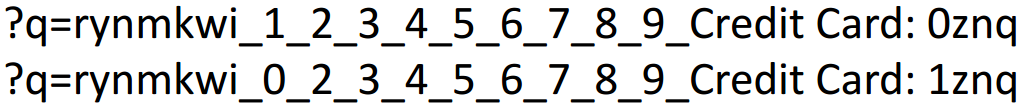
\includegraphics[width=0.8\textwidth]{diagrams/huffman_fixed_point.png}\end{figure}

In that case, the frequency of each letter is not affected from one request to
another, whereas rearranging the position allows us to perform the attack.

The above figure also depicts the use of random nonces before and after the main
body of the request, in this case \texttt{rynmkwi} and \texttt{znq}
respectively. These nonces are used to avoid the Huffman fixed-point prefix or
the character tested to be LZ77 compressed with strings before, in this case
\texttt{?q=}, or after the request and affect the consistency of the tests.

Our implementation of the methodology described is found in the request
initialization library \ref{sec:hillclimbing_py}. A user needs to input a chosen
prefix for the bootstrapping and an alphabet pool from some predefined alphabets
- uppercase letters, lowercase letters, decimal digits and dashes - as well as
serial or parallel method of attack. The functions of the library will then
create the appropriate request file that can be used along with the BREACH
script to issue the attack.

\section{Attack optimization}\label{sec:optimization}

The previous chapters have focused on expanding and explaining how the attack
could be a viable threat in real world applications. However, work still needs
to be done to make it faster and minimize the margin of error.

In this section we will describe two methods that improve the performance of the
attack, parallelization of hill-climbing and cross-domain parallelization.

\subsection{Parallelization of hill-climbing}

Up to this point, the characters of the alphabet are tested serially, one after
the other and again from top, when the end of the alphabet is reached. However,
a more efficient method could be followed, that could reduce the time of the
attack from \begin{math}O(|S|)\end{math} to \begin{math}O(log|S|)\end{math}.

The idea behind this method is based on the well-known
\texttt{divide-and-conquer} paradigm. Specifically, instead of using one test
character each time concatenated with the known prefix we could divide the
alphabet pool in half and issue requests on each such half. A request file
parameterized as such is the following:

\plaintext{File with parallelized request parameters.}{parallel_request.txt}

Using this method, for each step of the attack two different requests are made.
The first corresponds to one half of the alphabet and the second to the other
half. Whichever minimizes the length function should contain
the correct secret, so it is chosen and the same method applies to it until a
single character is chosen. That way we use binary searching techniques
dropping the attack factor noticeably.

The conditions for Huffman-induced noise and collateral compression are also met
here using the alphabet pool and the random nonces. Also in case of combined
alphabets such as lowercase letters, uppercase letters and digits, it is be
possible that biases are introduced regarding the different types, e.g.
lowercase letters could be better compressed than uppercase ones. We also bypass
this issue by dividing the alphabet alternately instead of consecutively.

\subsection{Cross-domain parallelization}

The tree structure of the Domain Name System
(DNS)\footnote{\url{https://en.wikipedia.org/wiki/Domain_Name_System}} defines
each non-resource record node as being a domain name. Each domain that is part
of a larger domain is called subdomain. Most websites use subdomains for
specific applications, that hold a certain role in the context of the basic web
application. Such applications include language versions of the website, mobile
versions or divisions of a larger organization such as Schools in a University
etc.

The existence of different subdomains can be used to make the attack more
efficient. In that case, multiple subdomains should handle same or similar data
containing the chosen secret. If cookies are available on the parent domain,
they are also available in the subdomains and can be used from the attacker.

Specifically different subdomains can resolve to different IPs, via DNS
poisoning. The source and destination IP information is included in the
Transport Layer of the network so it can be seen by an eavesdropper or, in our
case, the MitM proxy. The attack can be then issued on both domains effectively
parallelizing it with up to Nx efficiency, where N is the number of different
domains and subdomains.

\subsection{Point-system meta-predictor}\label{subsec:point_system}

Each variation of the attack so far assumed that after a number of requests
the mean length of the correct guess would be smaller than the length of each
incorrect. However, experiments conducted for the purpose of this work have
shown that this is not always the case.

In this section we introduce the concept of a meta-predictor, that employs a
point system in order to rank each guess compared to the others. The need for
such functionality became prominent, when it can be noticed that, although the
correct letter after an initial period until the attack is stabilized is among
the \textit{best} ones it is not necessarily \textit{the best} no matter how
many requests are made.

For that reason, we have created a point system, in order to evaluate the
performance of each letter in the context of a leatherboard of ascending mean
length order. This point system is declared in the constants' library
[\ref{sec:constants_py}] as below:

\begin{table}[H] \centering \begin{tabular} { | l | l | } \hline \textbf{1}: 20
& \textbf{2}: 16 \\ \textbf{3}: 12 & \textbf{4}: 10 \\ \textbf{5}: 8 &
\textbf{6}: 6 \\ \textbf{7}: 4 & \textbf{8}: 3 \\ \textbf{9}: 2 & \textbf{10}: 1
\\ \hline \end{tabular} \end{table}

Conceptually, it can be understood that the correct letter is more probable to
be among the \textit{best} ones over time even if it is not \textit{the best}
eventually compared to the others that will not be as \textit{good} in general,
although they may demonstrate a spike in performance for a certain period.

An example of this functionality against Facebook Chat is described extensively
in Section \ref{sec:fb_experiment}.

\chapter{Experimental results}\label{ch:experiment}

In this chapter we present the results of experiments, conducted in lab
environment, against two major systems, Facebook Chat and Gmail. We will analyze
the validity of the attack under different modes, serial and parallel, as well
as the time consumption of each method. Also, we will investigate the
effectiveness of the point-system meta-predictor, introduced in Section
\ref{subsec:point_system}.

\section{Facebook Chat messages}\label{sec:fb_experiment}

The first experiment targeted Facebook Chat, trying to exploit the vulnerability
presented in Section \ref{subsec:fb}. The first attempt used a regulat Facebook
account, with hundreds of friends and regular chat conversations and
notifications. However, using the validation method of Section
\ref{sec:mitmproxy}, it was found that between the secret and the reflection
lied a large amount of data, which led to a non-compression of the two, since
the LZ77 was not sufficient.

For that matter of this paper we have created a lab account, that has no friends
and no user activity of any kind, except for a self-sent private message, that
will be the secret to be stolen. That way, the noise of a real-world account,
such as new messages or notifications, is contained and we can avoid the
problems described above.

We assume an attack on Facebook chat messages, following the serial method of
requests, knowing the secret consists of letters, either lowercase or uppercase.
In order to steal the first letter of the secret, we perform 4000 iterations of
requests, which translates to 4000 for each letter in the alphabet or, in other
words, \begin{math}4000*52=208000\end{math} requests in total. The normal time
interval between two requests was set to 4 seconds, in order to be sure that
overlapping stream can be distinguished. This has led to an overall
\begin{math}208000*4 = 832000\end{math} seconds, which roughly equals to 9 days.

The following figure shows the behaviour of the correct letter as the attack
evolved:

\begin{figure}[H] \caption{Correct letter length chart.}
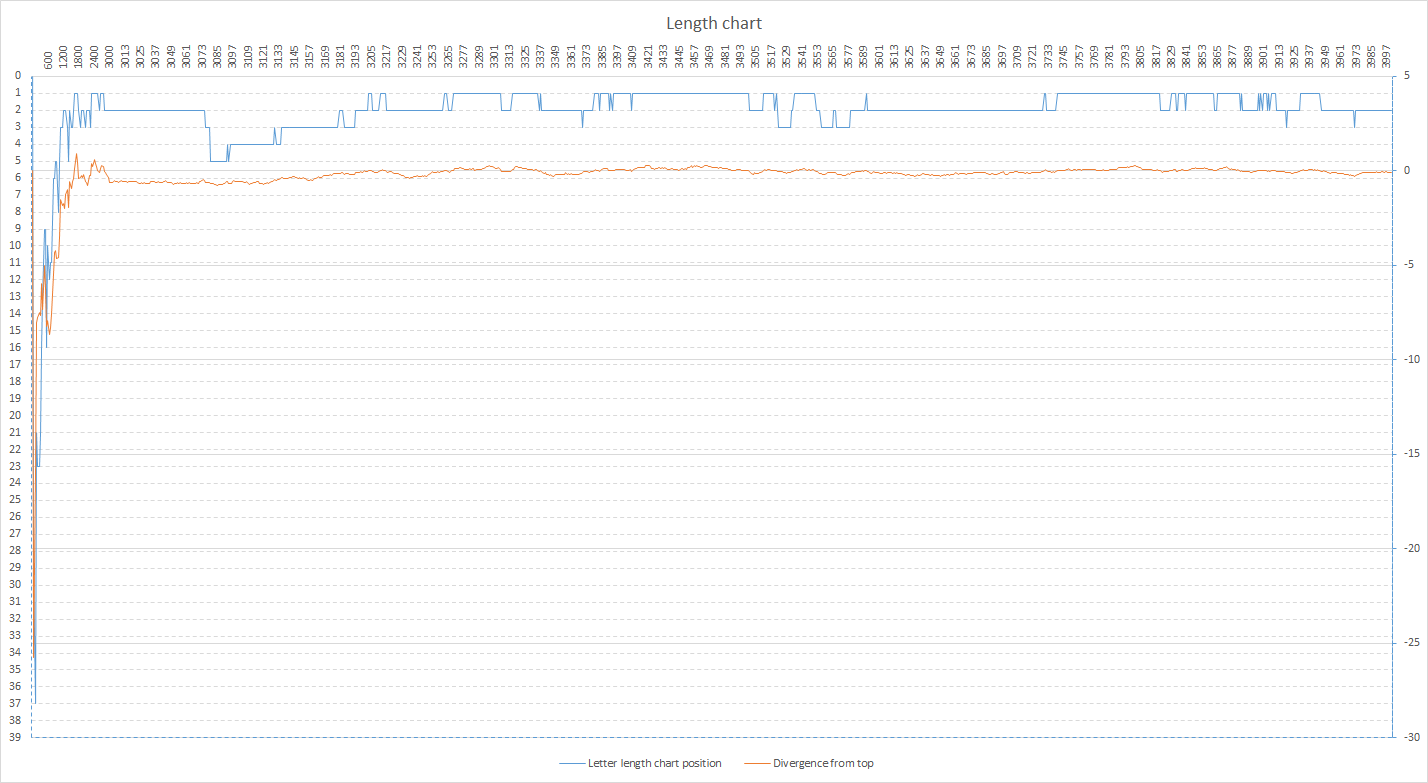
\includegraphics[width=1\textwidth]{diagrams/point_system_chart_1.png}\end{figure}

The top horizontal axis contains the number of iterations of requests.

The left vertical axis shows the position of the correct letter compared to the
others in ascending mean length order, i.e. the letter with minimum mean length
is \texttt{1}, the second smaller is \texttt{2} etc, and corresponds to the blue
curve.

The right vertical axis depicts the difference of the mean lengths of the
correct letter and the \textit{best} one, i.e. the one with minimum mean length,
or the second \textit{best}, in case the correct letter is the one of minimum
mean length.  This corresponds to the orange curve.

It can be understood that the correct guess presents a good behaviour after a
transient period, however, it does not always respond to the minimum mean
response length. In order to handle this problem, we introduced the point-system meta-predictor,
presented in Section \ref{subsec:point_system}. In a similar manner, we parsed
the collected data, using the point-system information.

The chart depicting the evolution of the correct letter's
behaviour in time, regarding the aggregated points, is shown in the following
figure:

\begin{figure}[H] \caption{Correct letter point chart.}
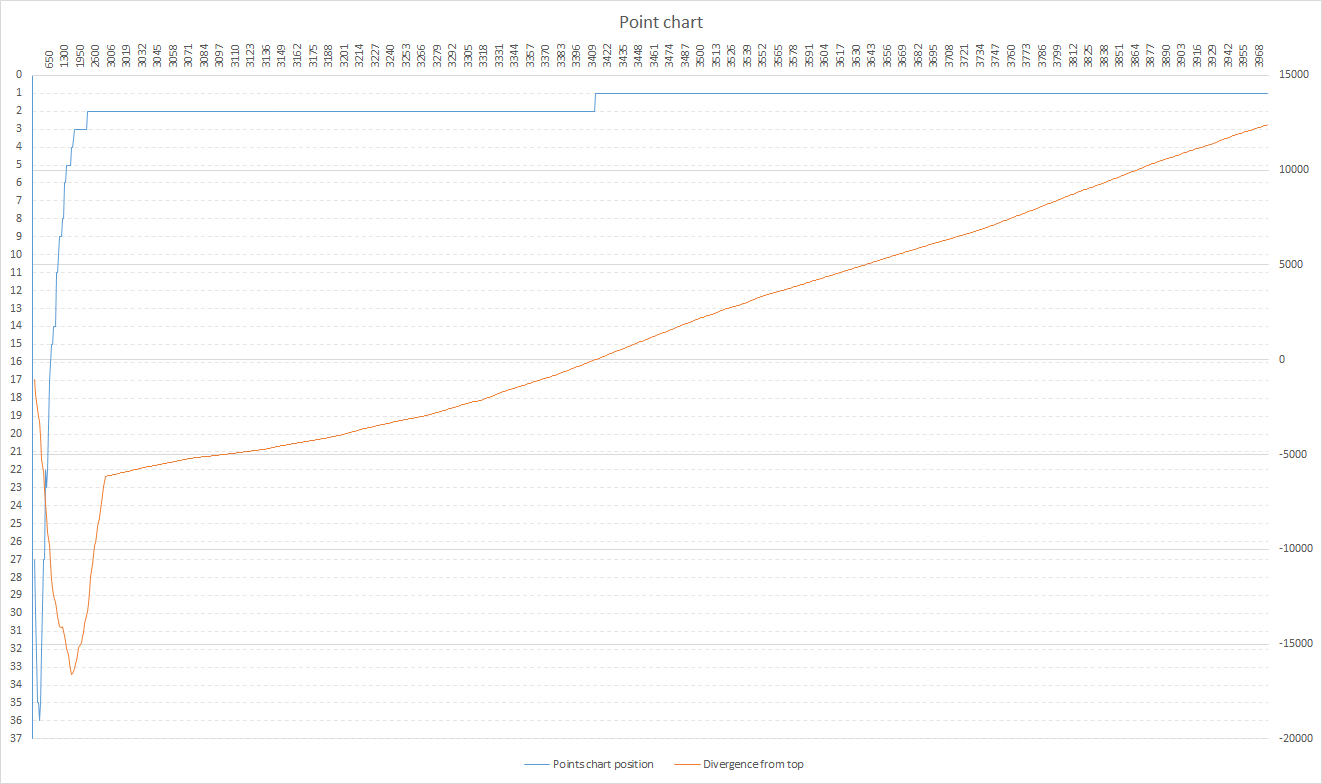
\includegraphics[width=1\textwidth]{diagrams/point_system_chart_2.png}\end{figure}

It is clear that, by introducing the point system, the prediction of the correct
letter is much more efficient than before. After a transient period, the correct
letter demonstrates a better behaviour compared to any other choice, increasing
its point performance in an almost linear rate over time.

The demonstrated attack provides a statistical proof that Facebook Chat is not
IND-PCPA. It is clear that an adversary could gain a major advantage in stealing a
private Facebook Chat message, using this attack model. However, it can be
understood that the attack performance of the attack is very limited, making it
particularly hard to be applied in real-world, where the conditions for success
would need to be applied for a noticeable period of time.

\section{Gmail Authentication token}\label{sec:gmail_experiment}



\chapter{Mitigation techniques}\label{ch:mitigation}

So far, this paper focused on the foundation and expansion of the attack. In
this chapter we will investigate several mitigation techniques. We will examine
the methods proposed by Gluck, Harris and Prado in the original paper under the
new findings that were described in previous chapters. Finally, we will propose
novel mitigation techniques, that either limit the scope of the attack or
eliminate it completely.

\section{Original mitigation tactics}\label{sec:original_mitigation}

The original BREACH paper \cite{breach} included several tactics for mitigating
the attack. In the following sections we will investigate them one by one, to
find if they can still be applied, after the findings of this work.

\subsection{Length hiding}

The first proposed method is an attempt to hide the length information from the
attacker. This can be done by adding a random amount of random data to the end
of the data stream for each response.

As stated in the BREACH paper, this method affects the attack efficiency only
slightly. Since the standard error of mean is inversely proportional to
\begin{math}\sqrt{N}\end{math}, where \begin{math}N\end{math} is the number of
repeated requests the attacker makes for each guess, the attacker can deduce the
true length with a few hundred or thousand requests.

In this paper we have described how repeated requests can lead to such bypassing
of the noise, as described in Section \ref{sec:probabilistic}.  Experimental
results have also shown that, for the endpoints tested, it is possible to
perform the attack under certain circumstances, despite of such noise.

\subsection{Separating Secrets from User Input}\label{subsec:sep_compression}

This approach states that user input and secrets are put in a completely
different compression context. Although this approach might work when the secret
is clearly distinct, it does not apply universally.

In this work, we were able to defeat this mitigation measure by introducing
alternative secrets. As described in Sections \ref{subsec:fb} and
\ref{subsec:gmail_mail}, user input and secrets are sometimes one and the same.
In the case of Facebook chat, the attacker can use as the chosen plaintext
private messages, and, in the case of Gmail, private mails.

In such cases, the secret and the attacker's chosen plaintext are
indistinguishable, making this mitigation technique inapplicable.

\subsection{Disabling Compression}

This paper focuses on attacks on encrypted compressed protocols. Since
encryption poses the vulnerability that is exploited, disabling it at the HTTP
level would result in total defeat of the attack.

However, such a solution would have drastic impact on the performance of web
applications. An example on Facebook, shows that a regular, empty search result
response page from a minimal account takes up to 12 kilobytes, if compressed,
opposed to 46 kilobytes, as raw plaintext. It is obvious that the trade-off is
too much to handle, especially for large websites that serve tens of thousands
of user requests per second.

\subsection{Masking Secrets}

The attacks investigated are based on the fact that the secret remains the same
between different requests. This mitigation method introduces a one-time pad
\begin{math}P\end{math}, that would be XOR-ed with the secret and concatenated
to the result, as follows \begin{math}P||(P \oplus S)\end{math}.

As we have found, Facebook uses this method in order to mask its CSRF tokens.
This successfully stops the attack from being able to steal this secret.

However, we have shown that many more secrets, other than CSRF tokens, exist,
that would need to be masked, in order to completely mitigate the attack. Since
masking doubles the length of every secret, while also making the secret not
compressible, due to the increase in entropy, the implementation of this method
would result in major loss of compressibility and, as a result, performance.

\subsection{Request Rate-Limiting and Monitoring}

The attack, especially against block ciphers, requires a large amount of
requests toward the chosen endpoint. In order for it to give results in a
reasonable amount of time, these requests would need to be made in a short
period. In such case, if the endpoint monitors the traffic from and to a
specific user and limits the requests to a certain amount for a specified time
window, it would slow down the attack significantly.

However, this method also does not come without cost. Rate limiting provides a
half-measure against the attack, since it only introduces a delay, without
defeating it completely. When more optimization techniques are proposed, like
the ones described in Section \ref{sec:optimization}, this delay would prove to
be of little help. On the other hand, rate limits may also introduce
\texttt{Denial-of-Service}\footnote{\url{https://en.wikipedia.org/wiki/Denial-of-service_attack}}
attacks against the victim.

\subsection{More Aggressive CSRF Protection}

As the original BREACH paper stated, "requiring a valid CSRF token for all
requests that reflect user input would defeat the attack".

While this is true for CSRF tokens, we have showed that alternative secrets,
that cannot be distinguished from user input, could still be compromised.

\section{Novel mitigation techniques}\label{sec:novel_mitigation}

In this section we propose several potentially stronger mitigation techniques,
that have not been introduced in literature so far.

\subsection{Compressibility annotation}\label{subsec:annotation}

As described in Section \ref{subsec:sep_compression}, a mitigation technique
could involve different compression implementations for secrets and user input.
Although, as we showed, this solution does not apply for all kinds of secrets,
it could be effective for most commonly and easily attacked ones, such as CSRF
tokens.

Our proposition is that web servers and web application servers cooperate to
indicate which portions of data must not be compressed. Application servers
should be parameterized by the user, in order to annotate each response to the
web server.

Annotation would then indicate where secrets are located and where a reflection
could be located. The annotation syntax could include HTML tags, that describe
the functionality of each data portion in the body of the response, a deployment
descriptor, such as \texttt{web.xml} used in Java applications, or a new special
format.

The annotated response from the application server would then be interpreted by
the web server, that would change its compression behavior accordingly.
Specifically, the server could disable compression of either reflections or
secrets or both, sending them always as literals. In case of BREACH, disabling
the LZ77 stage of compression would also be sufficient, since the functionality
of this algorithm is the one exploited in such attacks, whereas Huffman does
more harm than good.

Furthermore, this functionality should be implemented separately in every web
framework, such as Django\footnote{\url{https://www.djangoproject.com}}, Ruby on
Rails\footnote{\url{http://rubyonrails.org}} or
Laravel\footnote{\url{http://laravel.com}}, as well as web servers, such as
Apache\footnote{\url{http://httpd.apache.org}} or
Nginx\footnote{\url{http://nginx.org}}. In each framework a module should be
created, i.e. \texttt{mod\_breach}, that handles the annotation on either side
of the communication.

\subsection{SOS headers}\label{subsec:sos}

Storage Origin Security (SOS) is a policy proposed by Mike Shema and Vaagn
Toukharian in their 2013 Black Hat presentation \texttt{Dissecting CSRF Attacks
\& Defenses} \cite{sos}. Its intended purpose is to counter CSRF attacks,
however a side-effect would be the mitigation of attacks, such as BREACH.

SOS applies on cookies and defines whether a browser should include each cookie
during cross-origin requests or not. This definition is included in the
Content-Security-Policy response header of a web application, in a form that
sets a SOS policy for each cookie.

The policies applied are \texttt{any}, \texttt{self}, \texttt{isolate}.
\texttt{Any} states that the cookie should be included in the cross-origin
requests,  after a pre-flight request is made to check for an exception to the
policy. This is the behaviour browsers show as of today. \texttt{Self} states
that the cookie should not be included, although again a pre-flight request is
issued to check for exceptions. \texttt{Isolate} states that the cookie should
not be included in any case and no pre-flight request should be made.

Pre-flight requests are already used extensively under the Cross-origin resource
sharing
(CORS)\footnote{\url{https://en.wikipedia.org/wiki/Cross-origin_resource_sharing}}
standard.  This mechanism describes HTTP headers, that allow browsers to request
remote URLs only if they have permission. The browser sends a request that
contains an \texttt{Origin} HTTP header, to which the server responds with a
list of origin sites, that are allowed to access the content, or an error page,
in case cross-origin is prohibited.

SOS policy introduces a \texttt{Access-Control-SOS} header, which includes a
list of cookies that the browser needs to confirm, before including in the
request. The server could then respond with a \texttt{Access-Control-SOS-Reply}
header, that instructs the browser to \texttt{allow} or \texttt{deny} all of the
cookies mentioned in the request header, as well as a timeout period for the
browser to apply this new policy. In absence of such a reply header, the browser
may apply the default policy of each cookie instead.

BREACH relies on cross-origin requests, in order for the attacker to insert a
chosen plaintext in the body of a response from a chosen endpoint. The
introduction of SOS headers would effectively stop BREACH and similar future
attacks, that exploit this aspect of web communications.

If SOS method were to be applied, websites could apply strict policies, as to
which origins could access which data and under which context. As long as
websites integrate HTTP Strict Transport Security
(HSTS)\footnote{\url{https://en.wikipedia.org/wiki/HTTP_Strict_Transport_Security}},
malicious script injection, as described in Section \ref{sec:persistence}, would
be counter-measured. Combined with SOS headers, a malicious website, controlled
by the attacker, could be disallowed from issuing requests including the
victim's cookies, resulting in practical mitigation against partially chosen
plaintext attacks, such as BREACH.

For more information regarding SOS headers we refer to Black Hat presentation
slides
\footnote{\url{https://deadliestwebattacks.files.wordpress.com/2013/08/bhus_2013_shema_toukharian.pdf}}
and video \footnote{\url{https://www.youtube.com/watch?v=JUY4DQZ02o4}}, as well
as an extended blog post on the
proposal\footnote{\url{deadliestwebattacks.com/2013/08/08/and-they-have-a-plan/}}.
Also, there is a discussion thread in the mailing list of W3C Web Application
Security Working
Group\footnote{\url{http://lists.w3.org/Archives/Public/public-webappsec/2013Aug/0037.html}},
regarding the implementation of SOS headers as a standard in modern browsers.

\chapter{Conclusion}\label{conclusion}

\section{Concluding remarks}

Attacks on encrypted protocols, that exploit compression methods applied on the
plaintext handled by those protocols, such as BREACH, have only recently been
described.  Literature works so far show limited theoretical definitions of this
new type of attacks, while experimental results touch a relatively small scope
of protocols used nowadays.

This work focused on assessing the threat of such attacks for widely used
protocols, expanding the theoretical definition, as well as investigated the
success of methods designed for mitigation.

We introduced a cryptographical game for determining the property of
indistinguishability under partially chosen plaintext attacks. Also, we provided
intuitive proofs for comparison to other indistinguishability properties, along
with scenarios of application of partially chosen plaintext attacks on
compressed encrypted protocols.

The need for practical description of our method resulted in the definition of
an attack model, based on BREACH, that initiates, automates and validates the
attack. We also revealed major vulnerabilities on the two systems that we
experimented on, Facebook and Gmail, introducing new forms of secrets and chosen
plaintext an attacker could use.

In advance, we expanded the scope of the attack to block ciphers, we ulitized
various statistical methods, that bypass known obstacles, such as noise and
padding.  Furthermore, we proposed various optimization techniques that could
reduce the time and increase the efficiency of the attack, posing a valid threat
for real-world systems.

In order to perform experiments and validate the efficiency of the attack, we
implemented a framework in Python, that initiates the attack on a chosen
endpoint and parses the output in order to produce statistical results. From an
attacker's perspective, the framework must run on a machine inside the victim's
network, while the victim's machine is configured to send all traffic to the
endpoint to the attacker's machine and the victim also  browses a website
controlled by the attacker.

Experimental results have shown that, although the framework does not provide a
robust, bulletproof functionality, the attacker has a considerable advantage on
stealing a secret from the endpoints tested.

Finally, we investigated the ability of previously proposed mitigation
techniques to stop the attack under the findings, as well as proposed novel
methods that could effectively minimize the attack's success or even mitigate it
completely.

\section{Future Work}

Although this paper introduced the IND-PCPA property, formal definitions and
mathematical proofs should also be used to properly describe it. Also, this new
property should be formally evaluated, compared to other known properties.

As far as the practical attack is concerned, a consistency mechanism, as
described in Section \ref{sec:persistence}, is needed, in order to take full
advantage of vulnerabilities of simple HTTP connections. Furthermore, the
integration of MitM attacks, as the ones referenced in Section \ref{sec:mitm},
would result in a potential threat outside lab environment. It is also important
to implement a MitM proxy on TCP level, that would be able to distinguish
packets of different records, minimizing the margin of error for overlapping
response or request streams.

Finally, implementation of the two mitigation techniques, like proposed
compressibility annotation [\ref{subsec:annotation}] and SOS headers
[\ref{subsec:sos}], is vital in order to secure systems against attackst that
utilize the findings of this paper.

\chapter{Appendix}\label{ch:appendix}

\section{BREACH JavaScript}\label{sec:evil_js}

\jscode{evil.js}{evil.js}

\section{Request initialization library}\label{sec:hillclimbing_py}

\plaintext{hillclimbing.py}{hillclimbing.py}

\backmatter
\cleardoublepage % start at the next odd page
\phantomsection % correct hyperlinking
\bibliography{references}
\bibliographystyle{plain}
%\include{glossary}

\end{document}
